\section{Experiments}
\label{sec:eval}

We conducted experiments with an Apple M2 Pro chip and 32GB of RAM. All programs were implemented in C/C++.

\paragraph{\textbf{Datasets. }}
We generate synthetic datasets with independent, uniformly distributed attributes using the skyline data generator~\cite{borzsony2001skyline}.

We also evaluate five high-dimensional real datasets: NBA~\cite{basketballReference}, with $4{,}790$ player-season tuples and $104$ attributes; Car~\cite{epaAutomotiveTrends}, with $5{,}500$ vehicles and $57$ attributes; House~\cite{house_austin}, with $15{,}171$ properties and $33$ attributes; Energy~\cite{large-scale_wave_energy_farm_882}, with $36{,}043$ wave-energy farm configurations and $149$ attributes; and Activity~\cite{pamap2_physical_activity_monitoring_231}, with $2{,}872{,}533$ processed activity profiles and $54$ attributes. Detailed statistics appear in \iftoggle{TechnicalReport}{Section~\ref{appen:setting} of the \technicalreport}{Appendix~\ref{appen:setting}}.

We encoded missing values using the minimum observed value of the corresponding attribute. We removed constant attributes and normalized the remaining attributes to $[0,1]$, reversing those for which smaller values are preferred, as described in Section~\ref{sec:def}. All reported dimensionalities refer to the retained attributes.

\paragraph{\textbf{Algorithms. }}
We compare \textsc{FHDR} with two baselines: (1) \textsc{UtilityApprox}~\cite{NL12}, an interactive method applicable to high-dimensional data; and (2) \textsc{Sphere-Adapt}, an adaptation of the single-round \textsc{Sphere} algorithm~\cite{XW18}. For the set-output experiments, we adapt \textsc{UtilityApprox} to return the $K$ highest-scoring tuples under its estimated utility vector. To ensure fairness, \textsc{Sphere-Adapt} receives the candidate attribute set obtained by FHDR’s dimension reduction process and runs \textsc{Sphere} on the corresponding projected data. This comparison evaluates \textsc{AttributeSubset} against \textsc{Sphere} within the same discovered attribute space.

Table~\ref{tab:capabilities} summarizes the practical limitations of additional methods. In the tested high-dimensional settings, \textsc{UH-Random}/\textsc{UH-Simplex} and \textsc{HD-PI} encounter convex-hull computation failures, while \textsc{Verify-Point} encounters Qhull errors and excessive memory use. \textsc{Breakpoint} requires a counter repair on the large synthetic input and incurs substantial interaction and output costs. Detailed reproduction results are provided in \iftoggle{TechnicalReport}{Section~\ref{appen:capabilities} of the \technicalreport}{Appendix~\ref{appen:capabilities}}. We retain \textsc{UtilityApprox} and \textsc{Sphere-Adapt} for quantitative comparison and evaluate \textsc{UH-Random}’s upfront attribute-selection mechanism in the user study in Section~\ref{sec:user_study}.

\paragraph{\textbf{Parameter Setting. }}
We evaluate each algorithm by varying five key parameters: (1) dataset size $n$, (2) dimensionality $d$, (3) number of key attributes $d_\text{int}$, (4) number of answered questions $q$, and (5) output size $K$ for Problem~2~[\ref{p2}].

Unless otherwise specified, we use $d_\text{int}=3$~\cite{GG96, GA12, WX22, SC05, TK03, DMW12}, question size $s=2$~\cite{NL12}, question budget $q=15$ (see [\ref{q}] for justification), output size $K=30$~\cite{XW18}, and target regret ratio $\varepsilon=0$ for \textsc{UH-Random}. For synthetic datasets, we set $n=10^5$~\cite{NL12, WWX21, XCL19, XW18} and $d=100$.

We study two cases: complete interaction and limited feedback, with $q=15$ or $q=0$. We also vary the maximum number of displayed attributes $m$ and the number sampled per \textsc{AttributeSubset} inner run $w$ on real datasets across different $d_\text{int}$. Based on these results, we use $m=7$ and $w=6$; further details appear in \iftoggle{TechnicalReport}{Section~\ref{appen:setting} of the \technicalreport}{Appendix~\ref{appen:setting}}.

\paragraph{\textbf{Performance Measurement. }}
We evaluate the algorithms using four metrics: (1) \textit{execution time}, the end-to-end time (excluding user response time) for the final output; (2) \textit{regret ratio}, the relative utility loss between the best returned tuple and the global optimum under the ground-truth utility function; (3) \textit{outperformance rate}, the fraction of repeated runs in which our algorithm achieves the lowest regret ratio, with ties broken by execution time; and (4) \textit{number of questions}, which measures user effort.

Each experiment is repeated $100$ times with independently generated utility functions, and we report the averages.

\subsection{Results on Synthetic Datasets}
We evaluate sufficient- and limited-feedback settings separately. All experimental curves labeled \textsc{Sphere} correspond to \textsc{Sphere-Adapt}, as defined above.

\subsubsection{Problem 1}[\ref{p1}]
\begin{figure*}[ht]
  \centering

  \begin{minipage}[t]{0.32\textwidth}
    \centering
    \renewcommand{\arraystretch}{1.2}
    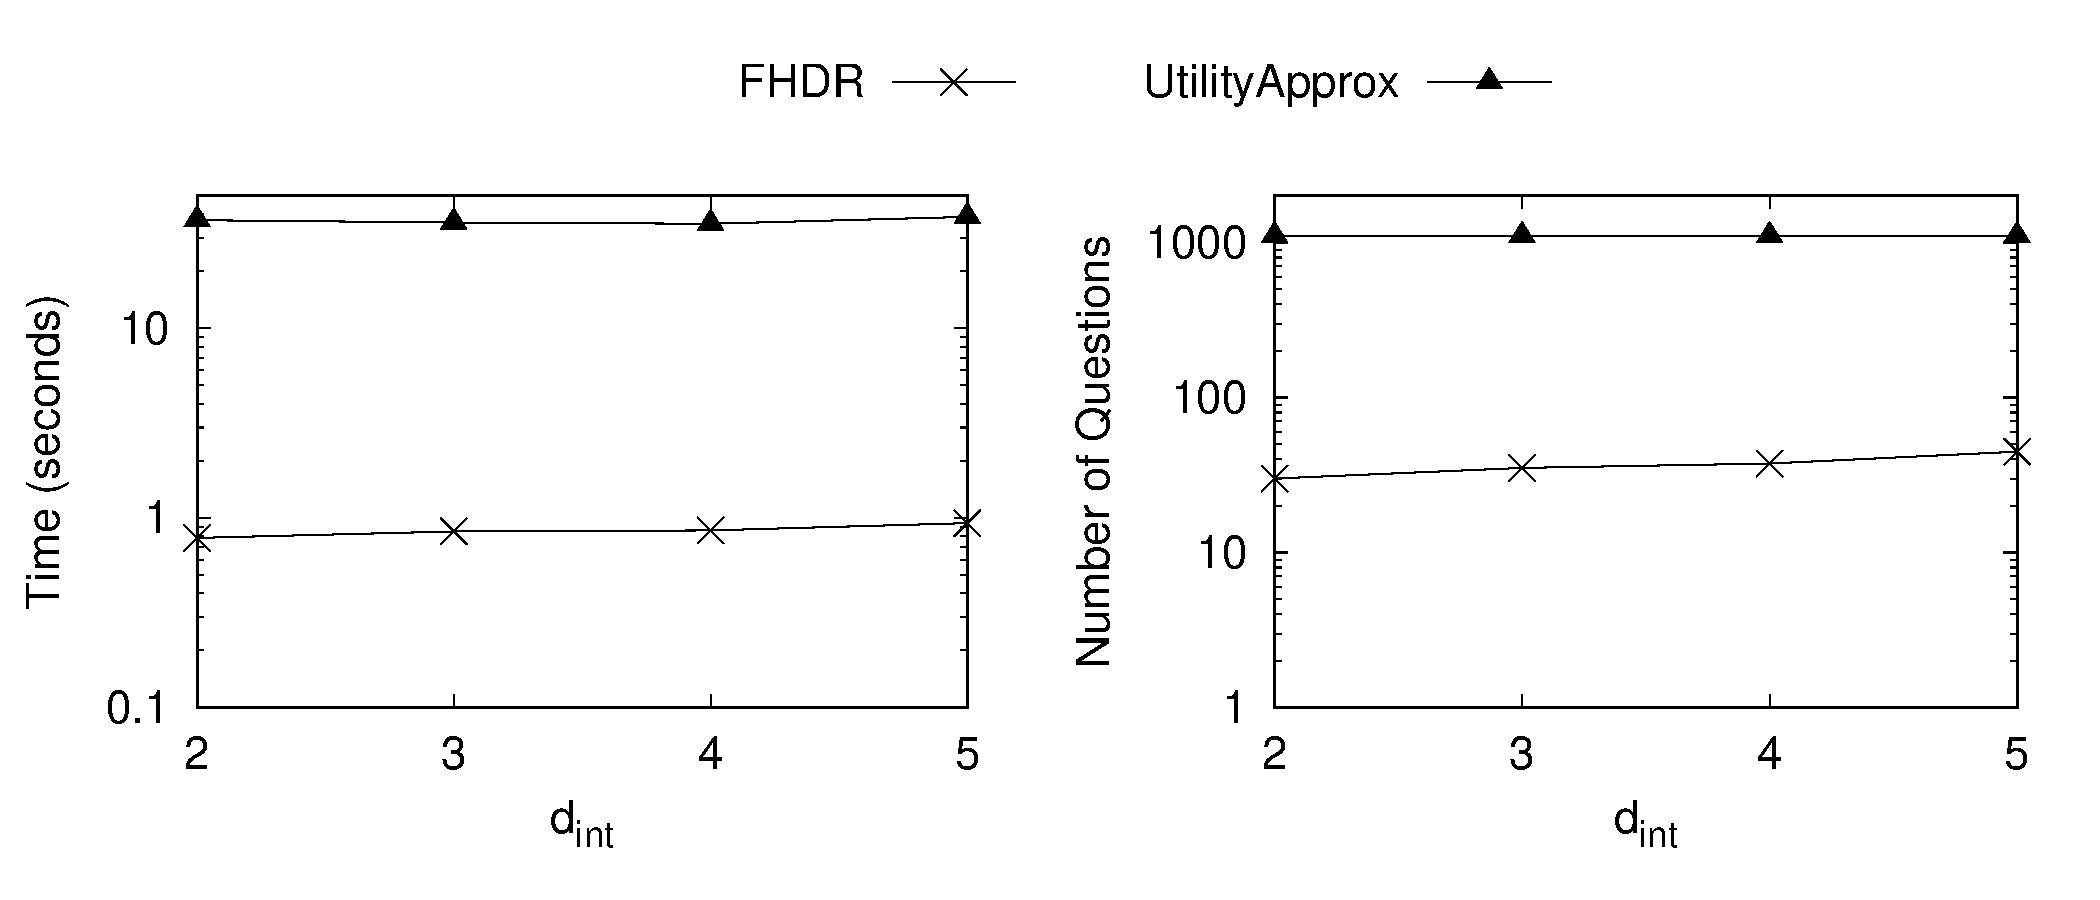
\includegraphics[width=\linewidth]{plot/p1/d_int_plots.pdf}
    \caption{P1: Vary $d_\text{int}$}
    \label{fig:p1_d_int}
  \end{minipage}
  \hfill
  \begin{minipage}[t]{0.32\textwidth}
    \centering
    \renewcommand{\arraystretch}{1.2}
    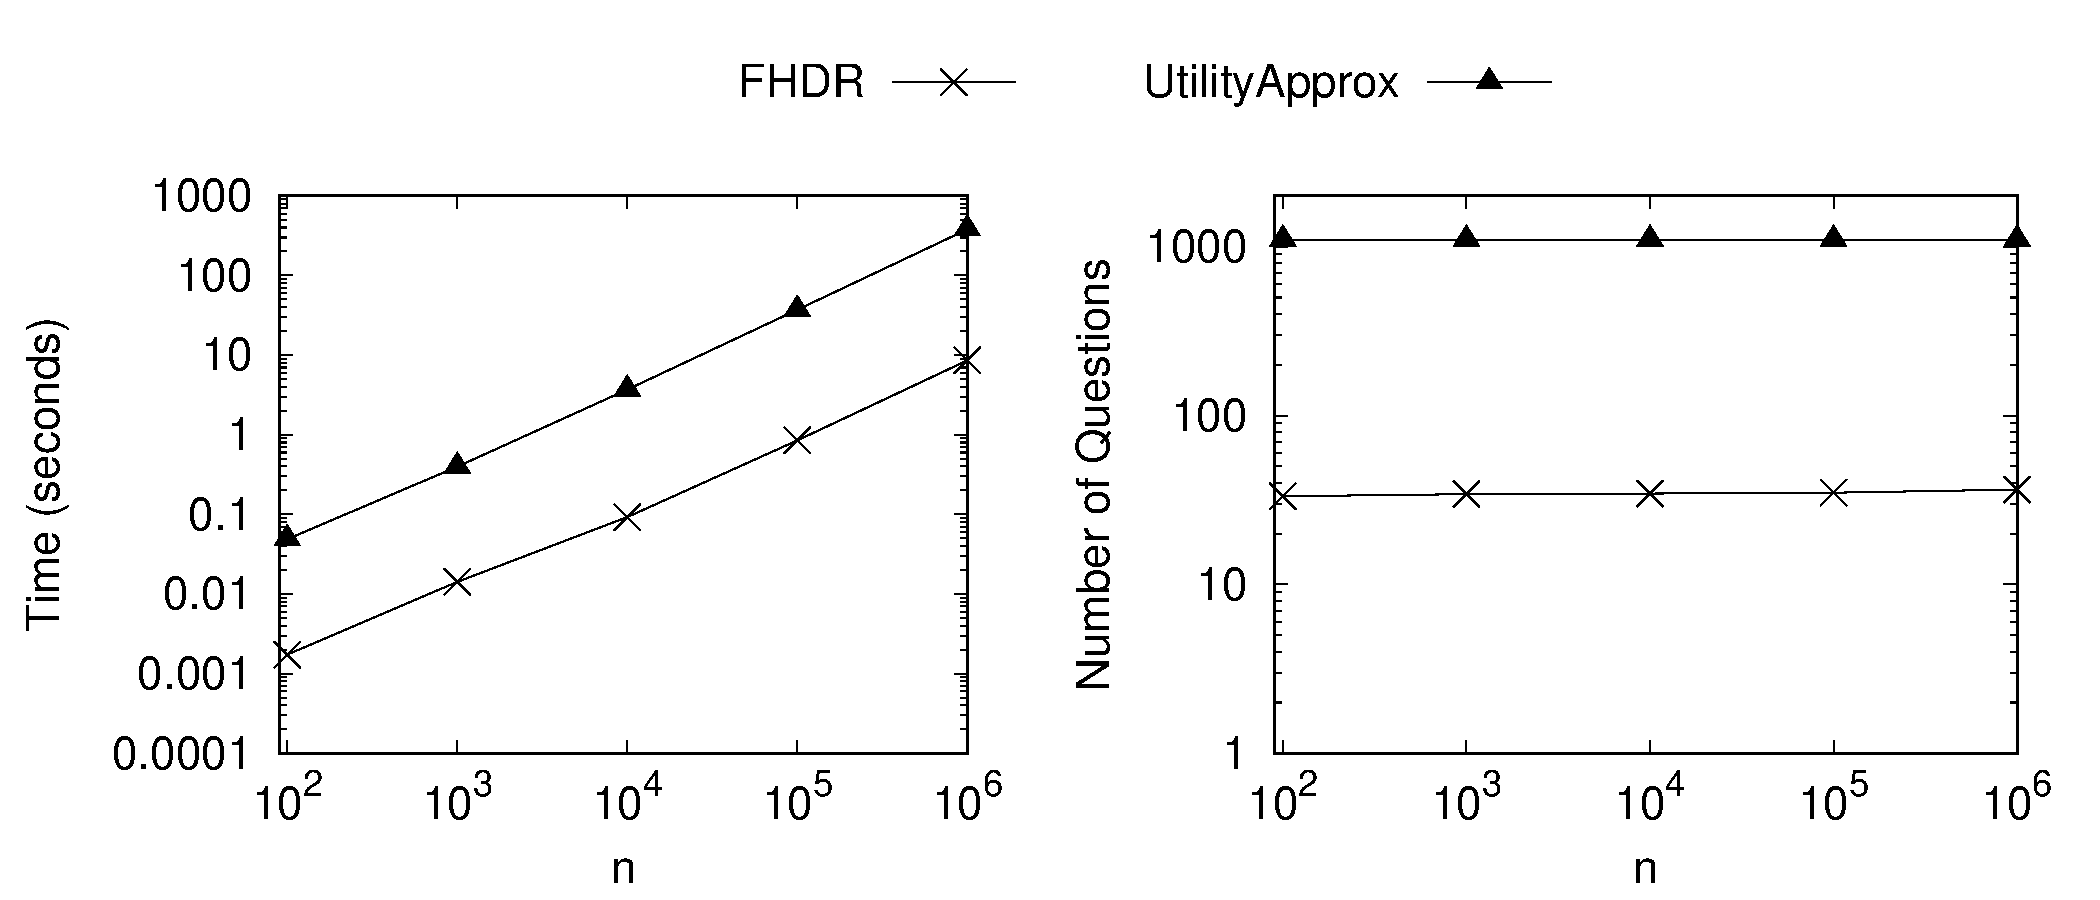
\includegraphics[width=\linewidth]{plot/p1/n_plots.pdf}
    \caption{P1: Vary $n$}
    \label{fig:p1_n}
  \end{minipage}
  \hfill
  \begin{minipage}[t]{0.32\textwidth}
    \centering
    \centering
    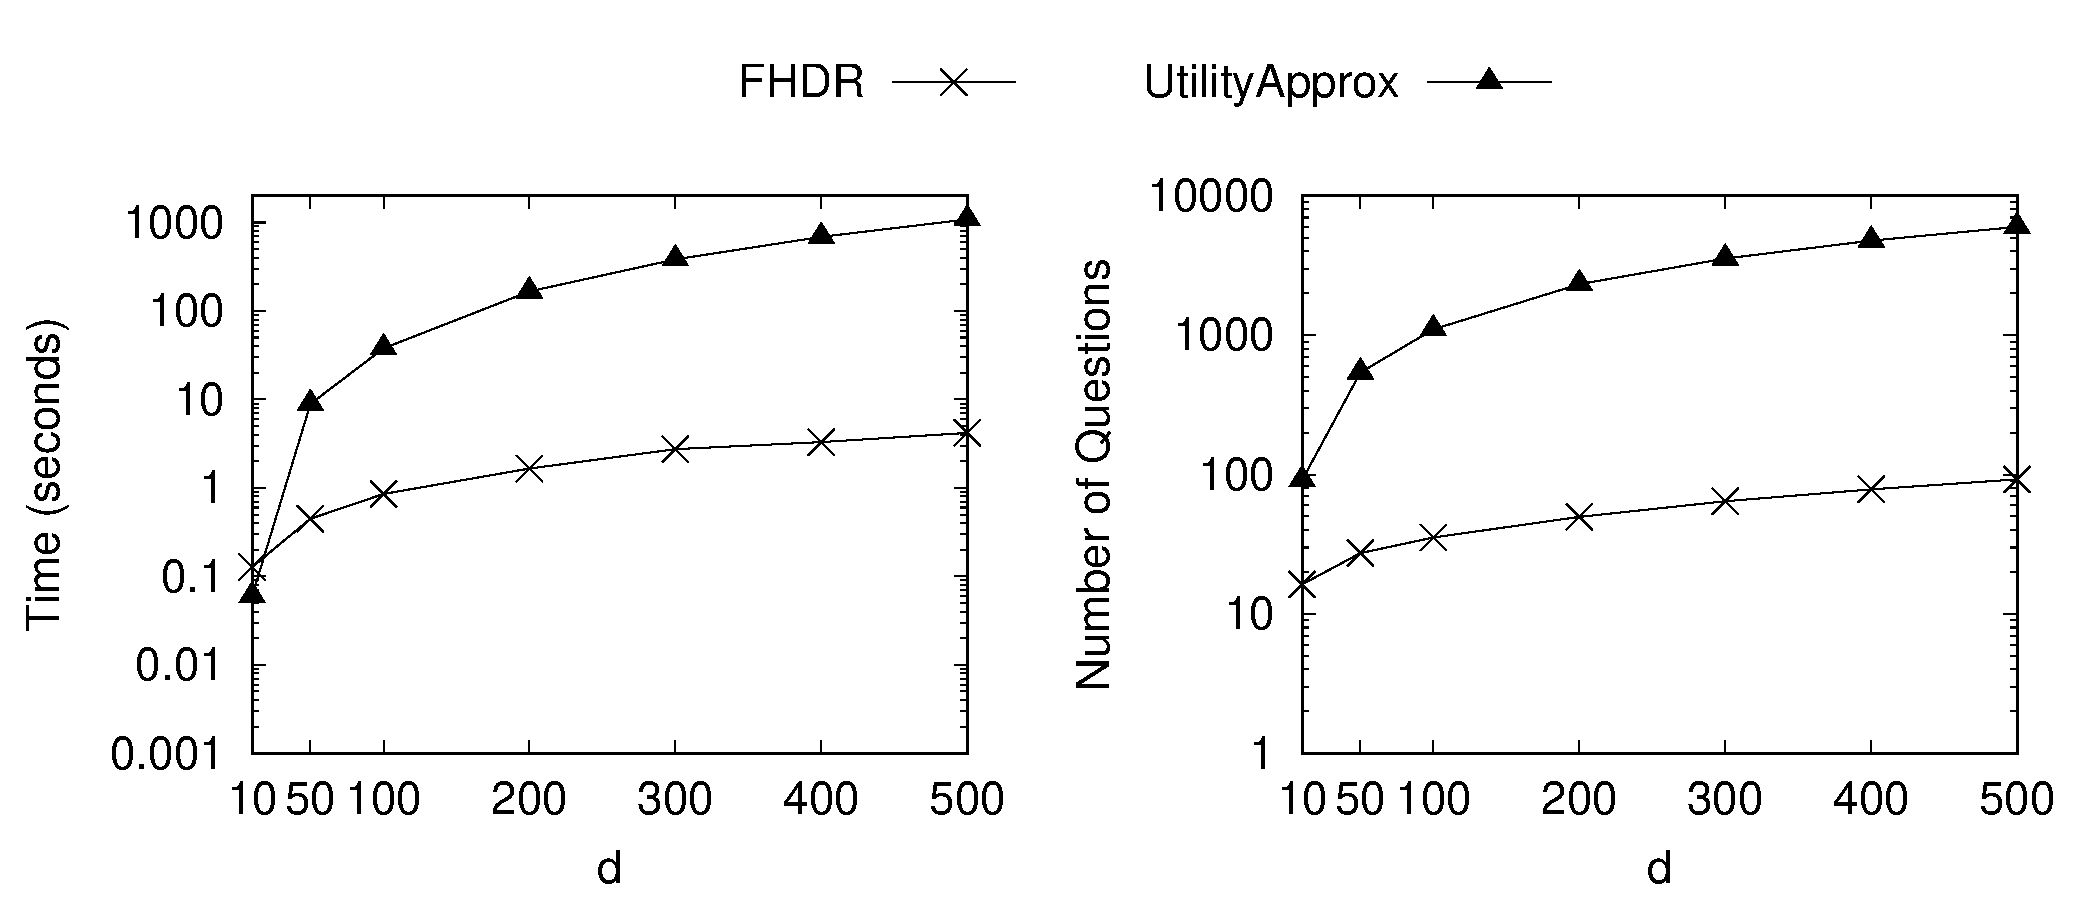
\includegraphics[width=\linewidth]{plot/p1/d_plots.pdf}
    \caption{P1: Vary $d$}
    \label{fig:p1_d}
  \end{minipage}

\end{figure*}

We first evaluate favorite-tuple retrieval under sufficient feedback, reporting the number of questions and execution time. FHDR terminates when its recommendation is certified as a favorite tuple. For \textsc{UtilityApprox}, we set $\varepsilon=0$ and terminate when $\sum_{i=1}^{d}(U_i-L_i)<10^{-9}$ or the $10{,}000$-question cap is reached, where $L_i$ and $U_i$ are its utility-coefficient bounds. Its reported costs correspond to this numerical convergence criterion. We compare with \textsc{UtilityApprox} here and evaluate the single-round \textsc{Sphere-Adapt} in the limited-feedback setting.

We vary the number of key attributes $d_\text{int}$ from $2$ to $5$, following the preference-sparsity setting motivated above. As shown in Figure~\ref{fig:p1_d_int}, the number of questions required by our algorithm increases moderately from $29$ to $42$, whereas \textsc{UtilityApprox} consistently requires approximately $1100$ questions, making it impractical for real-world use. The execution time remains low, increasing only from $0.02$~s to $0.05$~s, while \textsc{UtilityApprox} requires approximately $37$~s. The nearly constant behavior of \textsc{UtilityApprox} follows from its weakly truthful design: it refines the hidden utility function using synthetic tuples rather than actual data points. Consequently, for a fixed dimensionality $d$, the number of questions is largely independent of the input dataset. With a fixed number of tuples, its execution time therefore also remains nearly constant.

Figures~\ref{fig:p1_n} and~\ref{fig:p1_d} evaluate scalability with respect to the number of tuples $n$ and the dimensionality $d$. As shown in Figure~\ref{fig:p1_n}, our algorithm scales well with $n$, completing within a few seconds even when $n=10^6$. In contrast, the execution time of \textsc{UtilityApprox} grows approximately linearly with $n$, reaching $378$~s at $n=10^6$. For fixed $d$, our algorithm requires approximately $34$ questions regardless of $n$, whereas \textsc{UtilityApprox} requires about $1100$. As $d$ increases from $10$ to $500$, FHDR's question count grows much more slowly than \textsc{UtilityApprox}'s. By comparison, \textsc{UtilityApprox} requires $91$ questions at $d=10$ and $5989$ questions at $d=500$. The execution-time results exhibit a similar trend.

\subsubsection{Problem 2}[\ref{p2}]

\begin{figure}[ht]
    \centering
    \begin{minipage}{\linewidth}
        \centering
        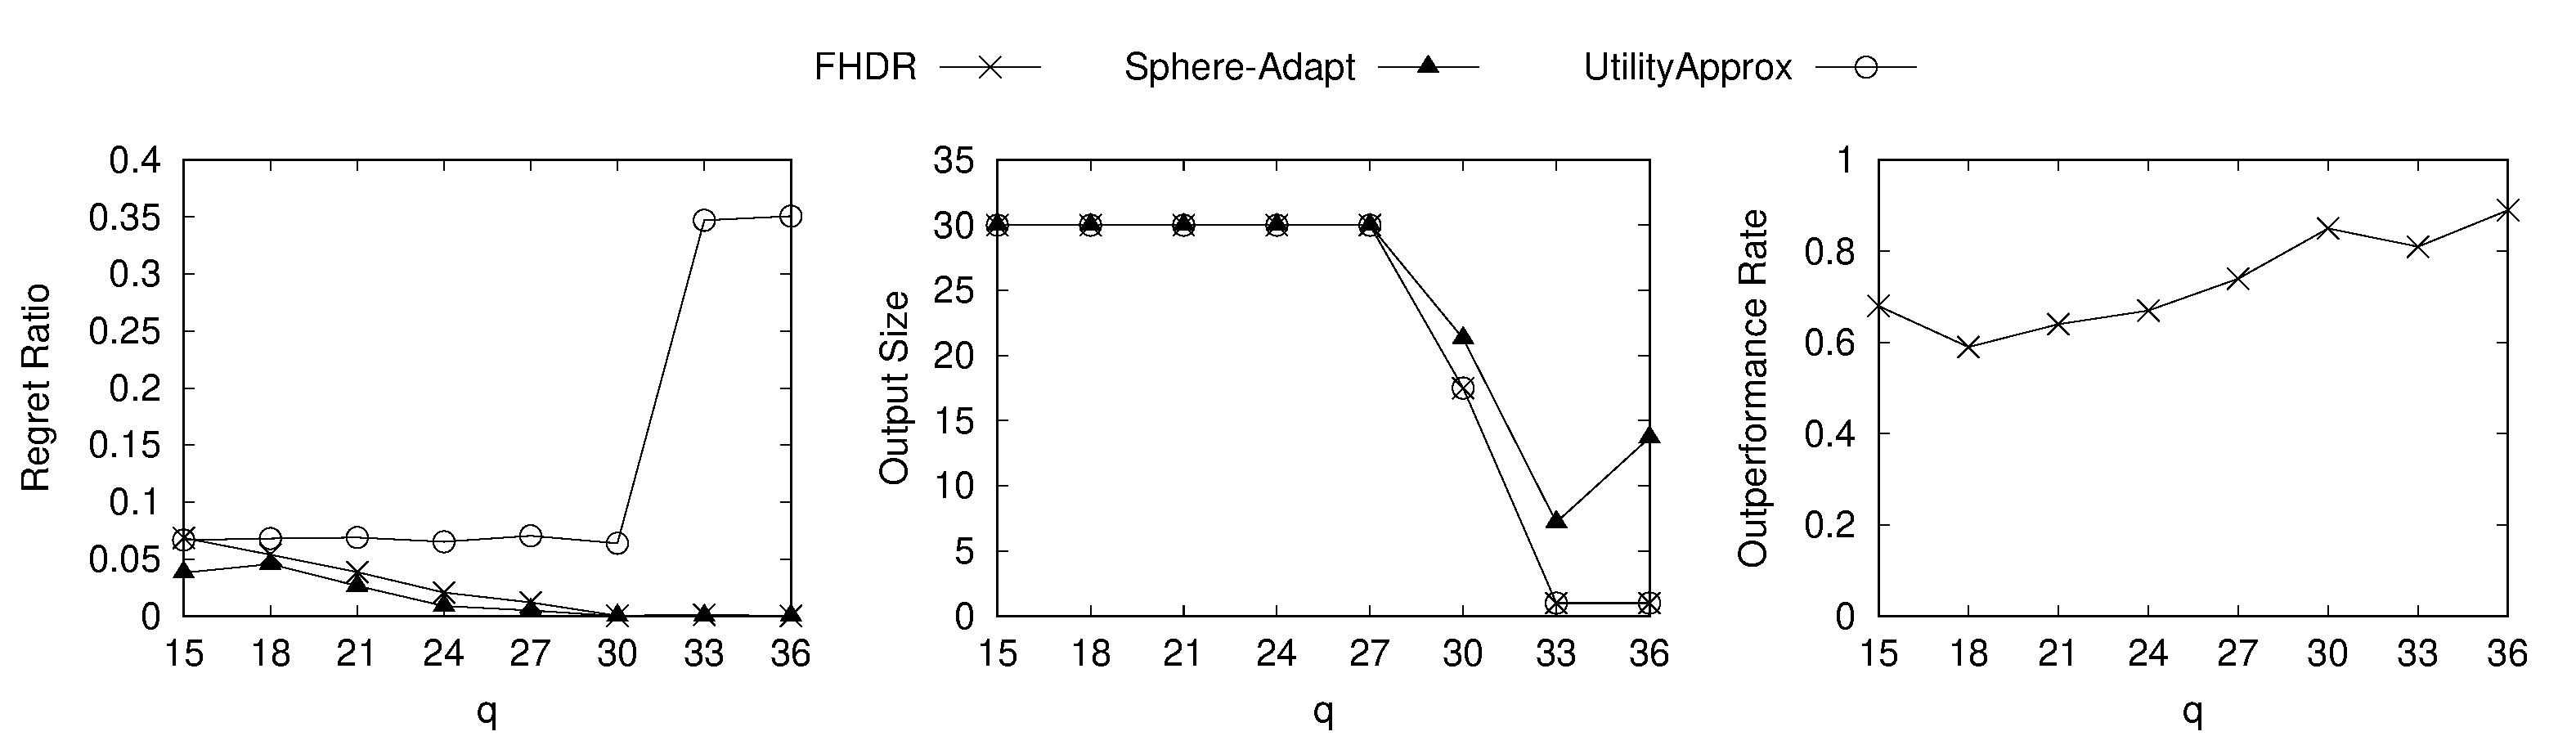
\includegraphics[width=\linewidth]{plot/p2/q_plots.pdf}
        \vspace{-1em}
        \caption{P2: Vary $q$}
        \label{fig:p2_q}
    \end{minipage}

    \begin{minipage}{\linewidth}
        \centering
        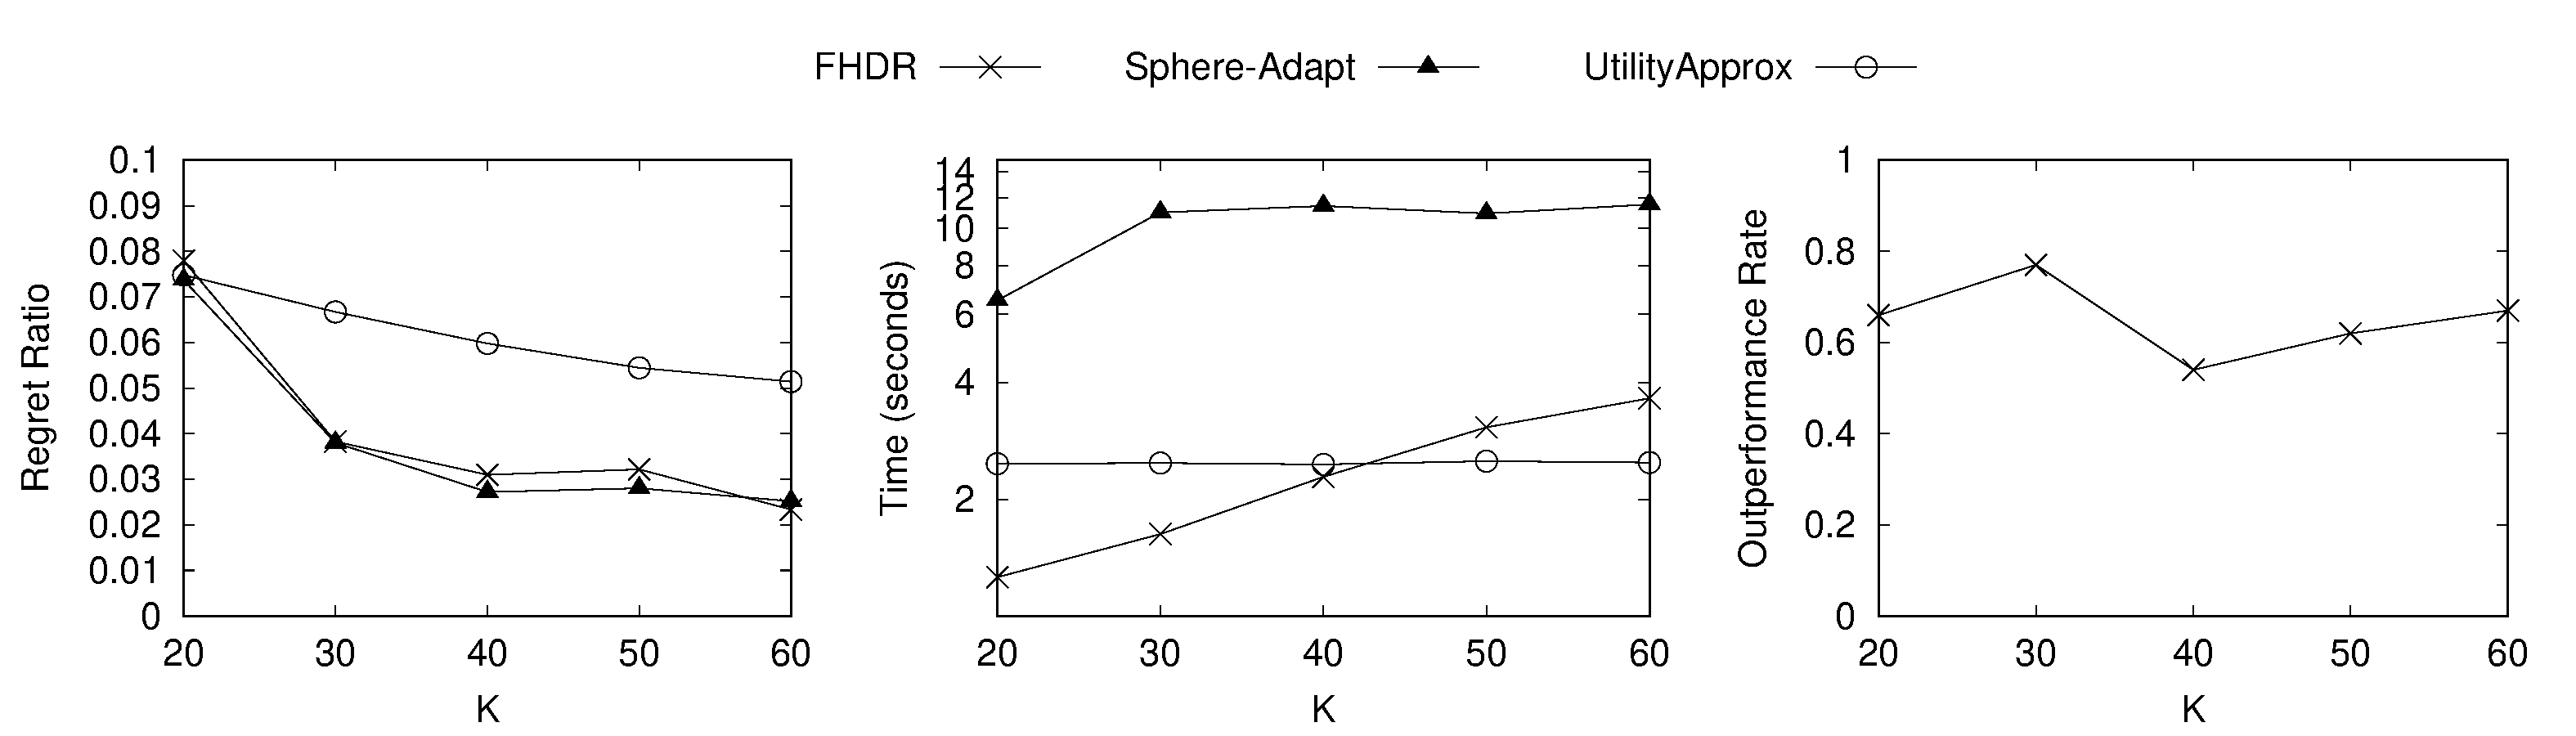
\includegraphics[width=\linewidth]{plot/p2/K_plots.pdf}
        \vspace{-1em}
        \caption{P2: Vary $K$}
        \label{fig:p2_K}
    \end{minipage}
    
    \begin{minipage}{\linewidth}
        \centering
        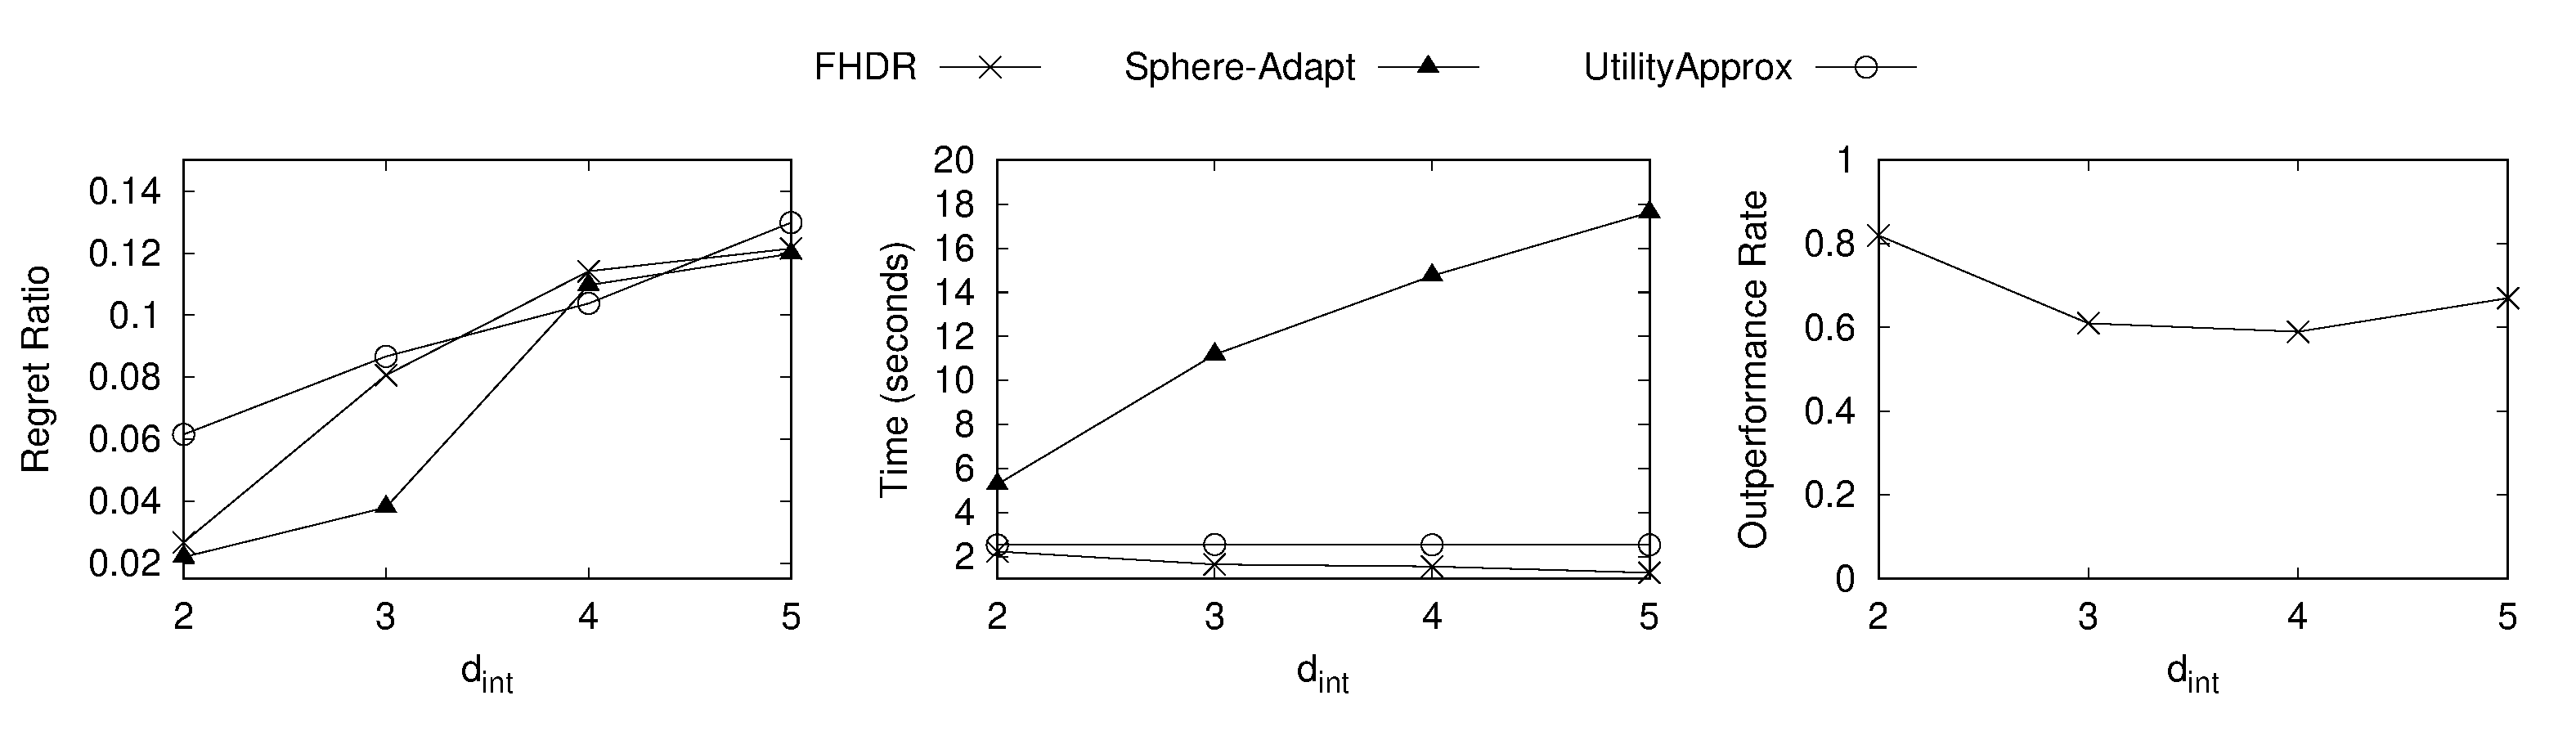
\includegraphics[width=\linewidth]{plot/p2/d_int_plots.pdf}
        \vspace{-1em}
        \caption{P2: Vary $d_\text{int}$}
        \label{fig:p2_d_int}
    \end{minipage}

    \begin{minipage}{\linewidth}
        \centering
        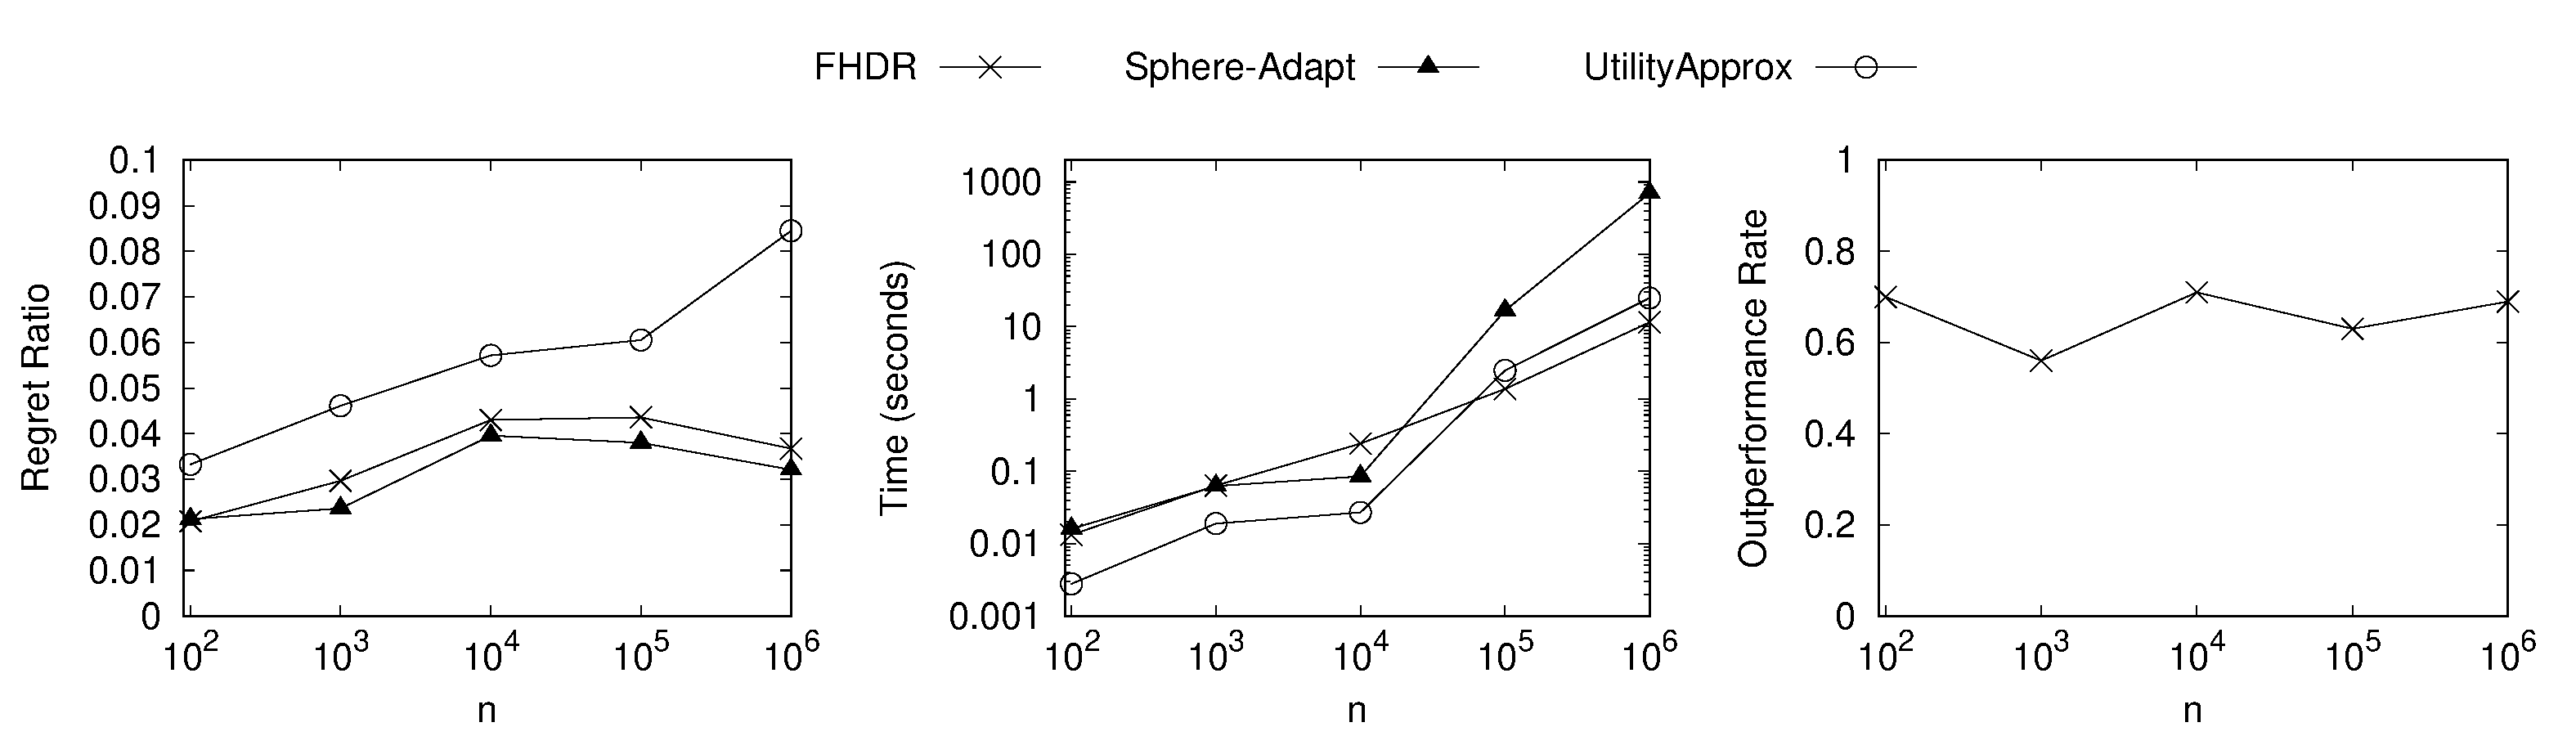
\includegraphics[width=\linewidth]{plot/p2/n_plots.pdf}
        \vspace{-1em}
        \caption{P2: Vary $n$}
        \label{fig:p2_n}
    \end{minipage}
    
    \begin{minipage}{\linewidth}
        \centering
        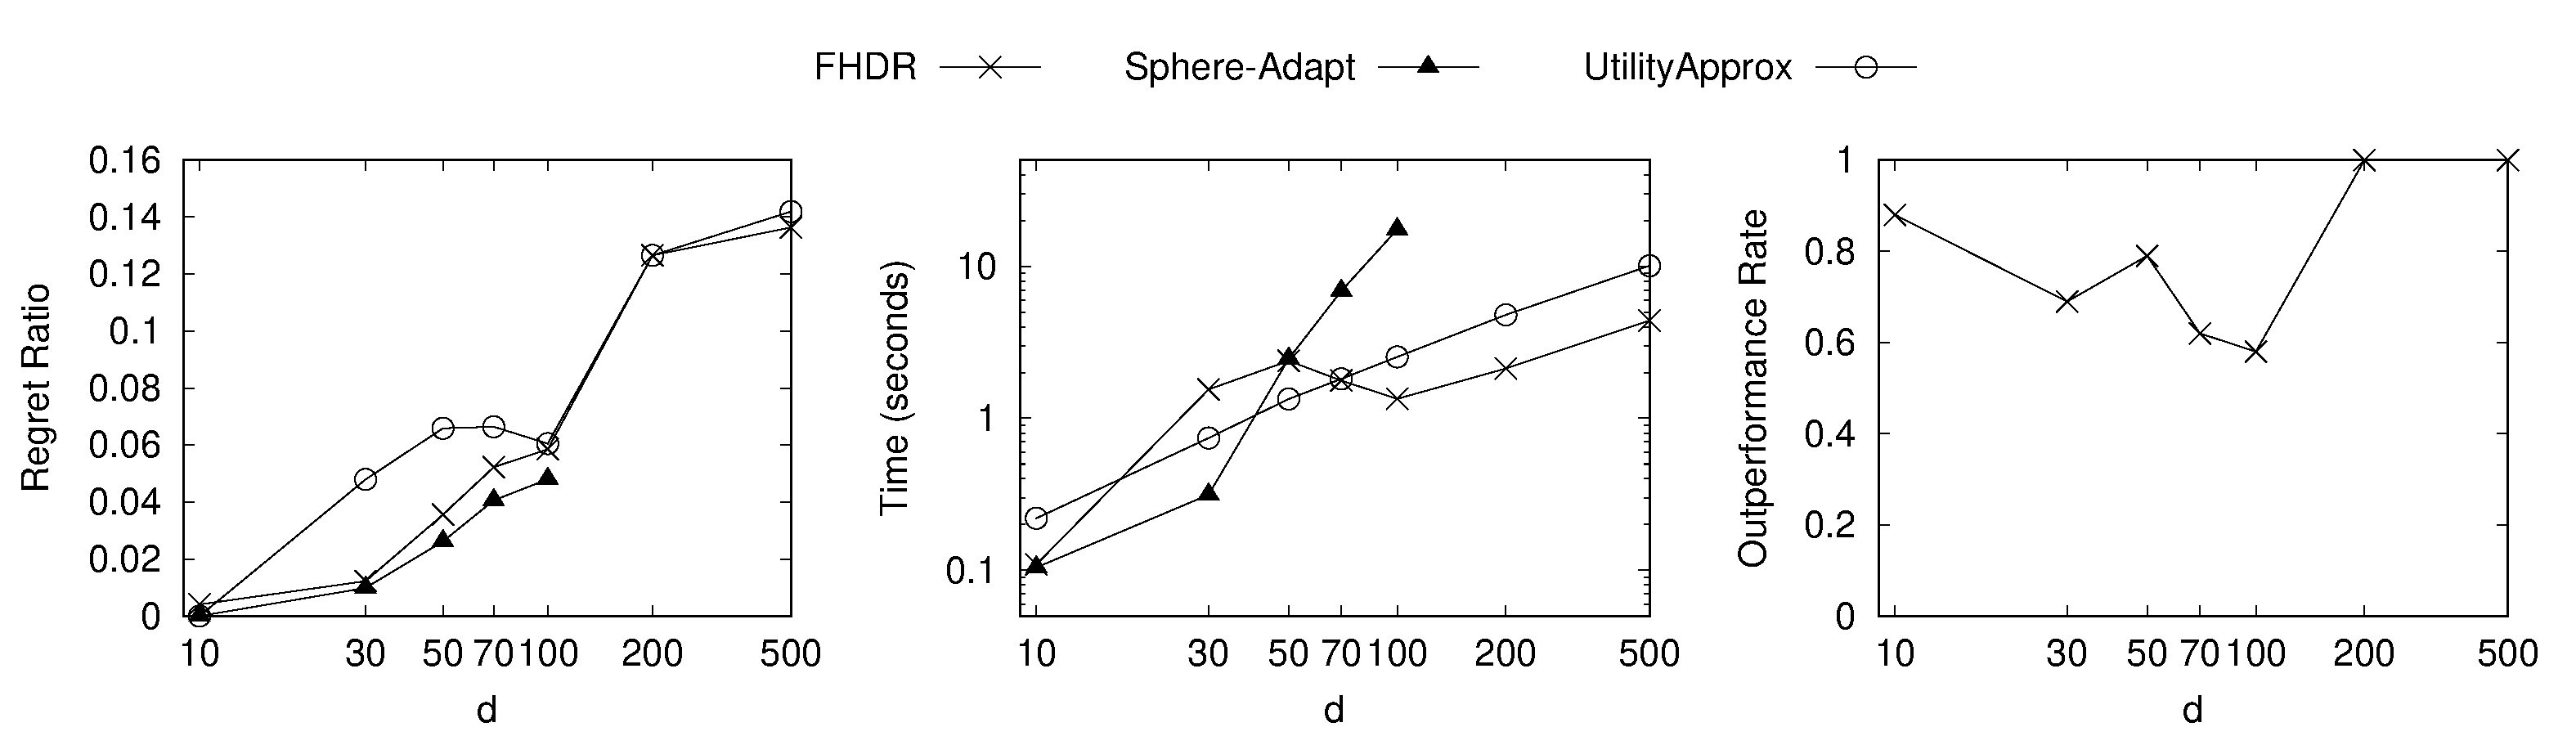
\includegraphics[width=\linewidth]{plot/p2/d_plots.pdf}
        \vspace{-1em}
        \caption{P2: Vary $d$}
        \label{fig:p2_d}
    \end{minipage}
    \begin{minipage}{\linewidth}
        \centering
        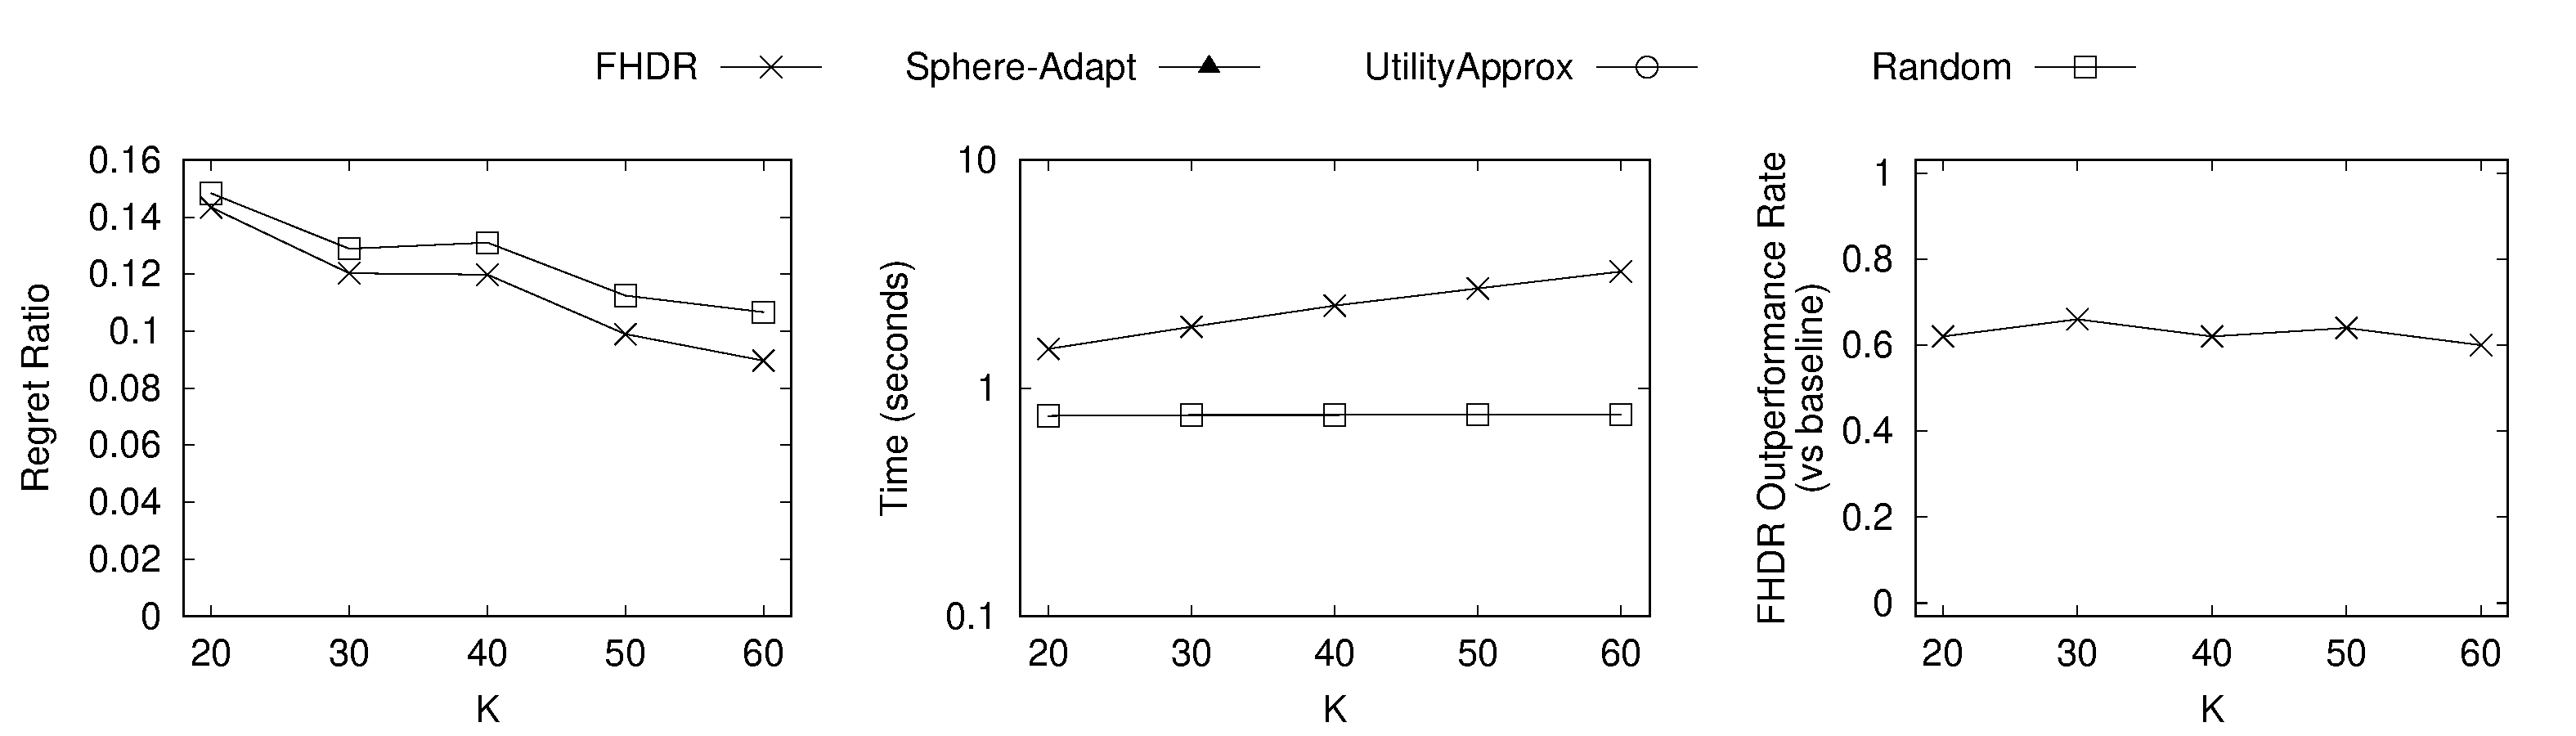
\includegraphics[width=\linewidth]{plot/p2_star/synthetic_K_plots.pdf}
        \vspace{-1em}
        \caption{$P2^{*}$: Vary $K$}
        \label{fig:p2star_synthetic}
    \end{minipage}
\end{figure}

We next evaluate recommendation quality under fixed question budgets.

\label{q}
Figure~\ref{fig:p2_q} varies $q$ from $15$ to $36$ in increments of $3$. Under the default settings, $15=\lceil100/7\rceil$ questions complete Phase 1 and leave at most $d_\text{int}m=21\leq K=30$ candidate attributes, allowing comparison with \textsc{Sphere-Adapt} under the same output budget.

Figure~\ref{fig:p2_q} shows FHDR reaching zero regret with sufficient Phase~3 feedback. Based on aforementioned algorithm design, if the user stops before Phase~3, FHDR returns a recommendation set; if interaction continues into Phase~3, FHDR returns one tuple and progressively refines the recommendation. Before FHDR enters the interactive Phase~3 branch, all methods return $K=30$ tuples. Afterward, FHDR and \textsc{UtilityApprox} return one tuple, while \textsc{Sphere-Adapt} uses the output budget $K=sq'$, where $q'$ counts FHDR’s additional Phase~3 questions and $s$ is the number of tuples displayed per question. Following the tuple-presentation accounting in~\cite{XCL19}, this budget gives the single-round method a corresponding allowance for FHDR’s additional interaction. \textsc{UtilityApprox}'s regret increase coincides with its output shrinking from $K=30$ tuples to one, as shown in the output-size panel. Returning fewer tuples can increase regret despite additional feedback; the curve therefore reflects changes in both the question budget and output size. Our method consistently achieves a lower regret ratio compared with \textsc{UtilityApprox}. While \textsc{Sphere-Adapt} attains similar regret ratios, our method performs better in over $60\%$ of cases.

We vary the output size $K$ in Figure~\ref{fig:p2_K}. FHDR achieves lower regret ratios than \textsc{UtilityApprox}. Its execution time increases from $1$ to $3$ seconds, compared with $\sim11$ seconds for \textsc{Sphere-Adapt}. Although slightly slower than \textsc{UtilityApprox}, it provides substantially better result quality and achieves the lowest regret ratio in $\sim60\%$ of the runs.

Figure~\ref{fig:p2_d_int} shows the effect of varying $d_\text{int}$, which reflects increasing preference complexity. For all three algorithms, the regret ratio grows approximately linearly as $d_\text{int}$ increases from $2$ to $5$, with lower regret observed at smaller values. Execution times remain consistent with earlier results, although our algorithm becomes slightly faster as $d_\text{int}$ increases. With a fixed question budget, a larger $d_\text{int}$ produces a larger candidate set $|\mathcal{D}_\text{cand}|$, reducing overlap among the inner output sets $S_i$. The union can therefore reach the fixed output size $K$ in fewer inner runs, reducing execution time.

Figures~\ref{fig:p2_n} and~\ref{fig:p2_d} evaluate scalability with respect to the number of tuples $n$ and dimensionality $d$. As $n$ increases, our algorithm maintains a regret ratio below $0.045$, substantially lower than \textsc{UtilityApprox}, whose regret increases noticeably. FHDR's runtime grows approximately linearly with $n$, whereas \textsc{Sphere-Adapt} scales less favorably. Section~\ref{sec:attsub} discusses \textsc{Sphere}'s dimension-dependent cost.

As shown in Figure~\ref{fig:p2_d}, our algorithm also consistently outperforms \textsc{UtilityApprox} in regret ratio and remains close to \textsc{Sphere-Adapt}. Its runtime stays within a few seconds, first peaking at $d=50$, then decreasing slightly before rising again. The temporary decrease occurs because a larger $d$ produces a larger candidate set $|\mathcal{D}_\text{cand}|$ under a fixed question budget, reducing overlap among the inner output sets and hence the number of \textsc{Sphere} runs within \textsc{AttributeSubset}. At larger $d$, dataset-loading costs begin to dominate. \textsc{Sphere-Adapt} becomes infeasible beyond $d=100$ under the default $K$ and $q$ settings, whereas our method continues to return valid results in approximately one second, demonstrating the robustness in extremely high-dimensional settings.

\paragraph*{Zero-Feedback Evaluation ($P2^{*}$)}
We also evaluate the special case of zero-feedback in Problem~2, denoted by $P2^{*}$, in which the user answers no questions ($q=0$). FHDR directly invokes \textsc{AttributeSubset} on all original attributes, without attribute elimination or elicited comparison constraints. We compare our method with \textsc{Random}, a baseline which samples $K$ distinct tuples uniformly without replacement from the entire dataset.

Figure~\ref{fig:p2star_synthetic} shows that FHDR achieves lower mean regret than \textsc{Random} at every tested $K$. As $K$ increases from $20$ to $60$, FHDR’s mean regret decreases from $0.1434$ to $0.0897$, compared with $0.1483$ to $0.1067$ for \textsc{Random}. FHDR achieves lower or equal regret in $60$--$66\%$ of runs.

\subsection{Results on Real Datasets}
We report NBA results for sufficient and limited feedback; results for the other real datasets appear in \iftoggle{TechnicalReport}{Section~\ref{appen:real} of the \technicalreport}{Appendix~\ref{appen:real}}.

For the case where the user answers all questions (Problem~1 (\ref{p1})), as \(d_{\text{int}}\) increases from 2 to 5, FHDR requires 30–40 questions and approximately 0.04 s, while UtilityApprox requires 1,149 questions (Figure~\ref{fig:nba_a}).

Figures~\ref{fig:nba_b}--\ref{fig:p2star_nba} report results for Problem~2, including its zero-feedback special case. For the positive-feedback experiments, we set the default budget to $q=\lceil d/m\rceil$, sufficient to complete Phase 1, following~\cite{LA24} and the synthetic-data setting. For NBA, this gives $q=15$. When varying $q$, we consider values from $\lceil d/m\rceil$ to the maximum number of questions observed across repeated runs for identifying the user’s favorite tuple.

Figure~\ref{fig:nba_b} evaluates the effect of varying $d_{\text{int}}$. \textsc{FHDR} achieves regret ratios comparable to \textsc{Sphere-Adapt} and lower than \textsc{UtilityApprox}. Its execution time decreases slightly from $0.08$ to $0.05$ seconds and remains lower than both baselines. On NBA, the smaller tuple count makes the absolute runtime difference less pronounced.

As \(K\) increases, regret decreases for all methods (Figure~\ref{fig:nba_c}). AttributeSubset achieves an outperformance rate of approximately 0.9 and runs faster than Sphere-Adapt. FHDR maintains low regret with only $15$ questions and reaches zero regret with sufficient feedback (Figure~\ref{fig:nba_d}). \textsc{UtilityApprox}'s regret increase again coincides with the reduction to singleton output under the evaluation protocol described above.

\paragraph*{Zero-feedback special case ($P2^{*}$)}
As shown in Figure~\ref{fig:p2star_nba}, FHDR’s mean regret is lower than \textsc{Random} by an order of magnitude. The quality advantage is greater than on the synthetic dataset: FHDR achieves lower or equal regret in $96$--$100\%$ of runs, with execution time all below $0.1$s. Thus, the zero-feedback advantage is more pronounced on NBA, with a small additional computation cost.

Across the evaluated real datasets, FHDR combines low regret with efficient execution and reduced interaction cost, consistent with the synthetic-data results. These findings support its practical effectiveness on high-dimensional real data.

\begin{figure}[ht]
    \centering
    \begin{subfigure}{\linewidth}
        \centering
        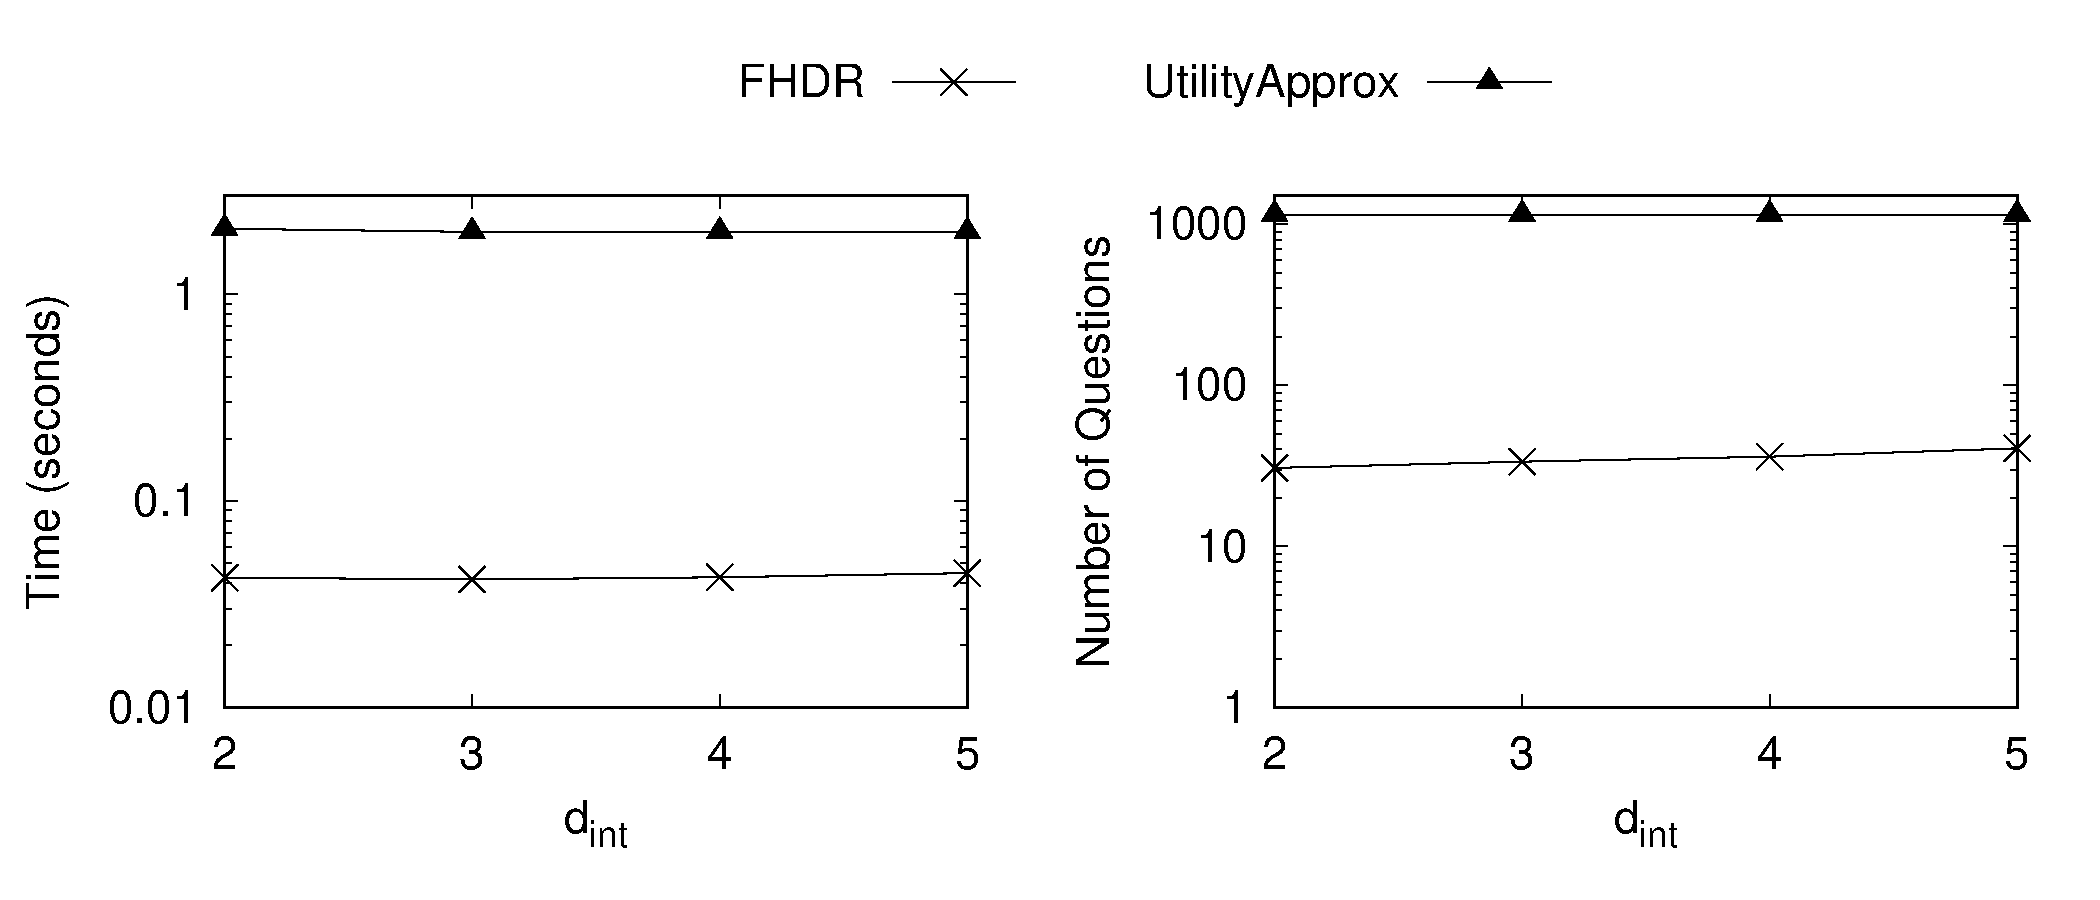
\includegraphics[width=0.67\linewidth]{plot/real/nba/d_int_1_plots.pdf}
        \vspace{-0.5em}
        \caption{P1: Vary $d_{\text{int}}$}
        \label{fig:nba_a}
      \end{subfigure}

    \begin{subfigure}{\linewidth}
        \centering
        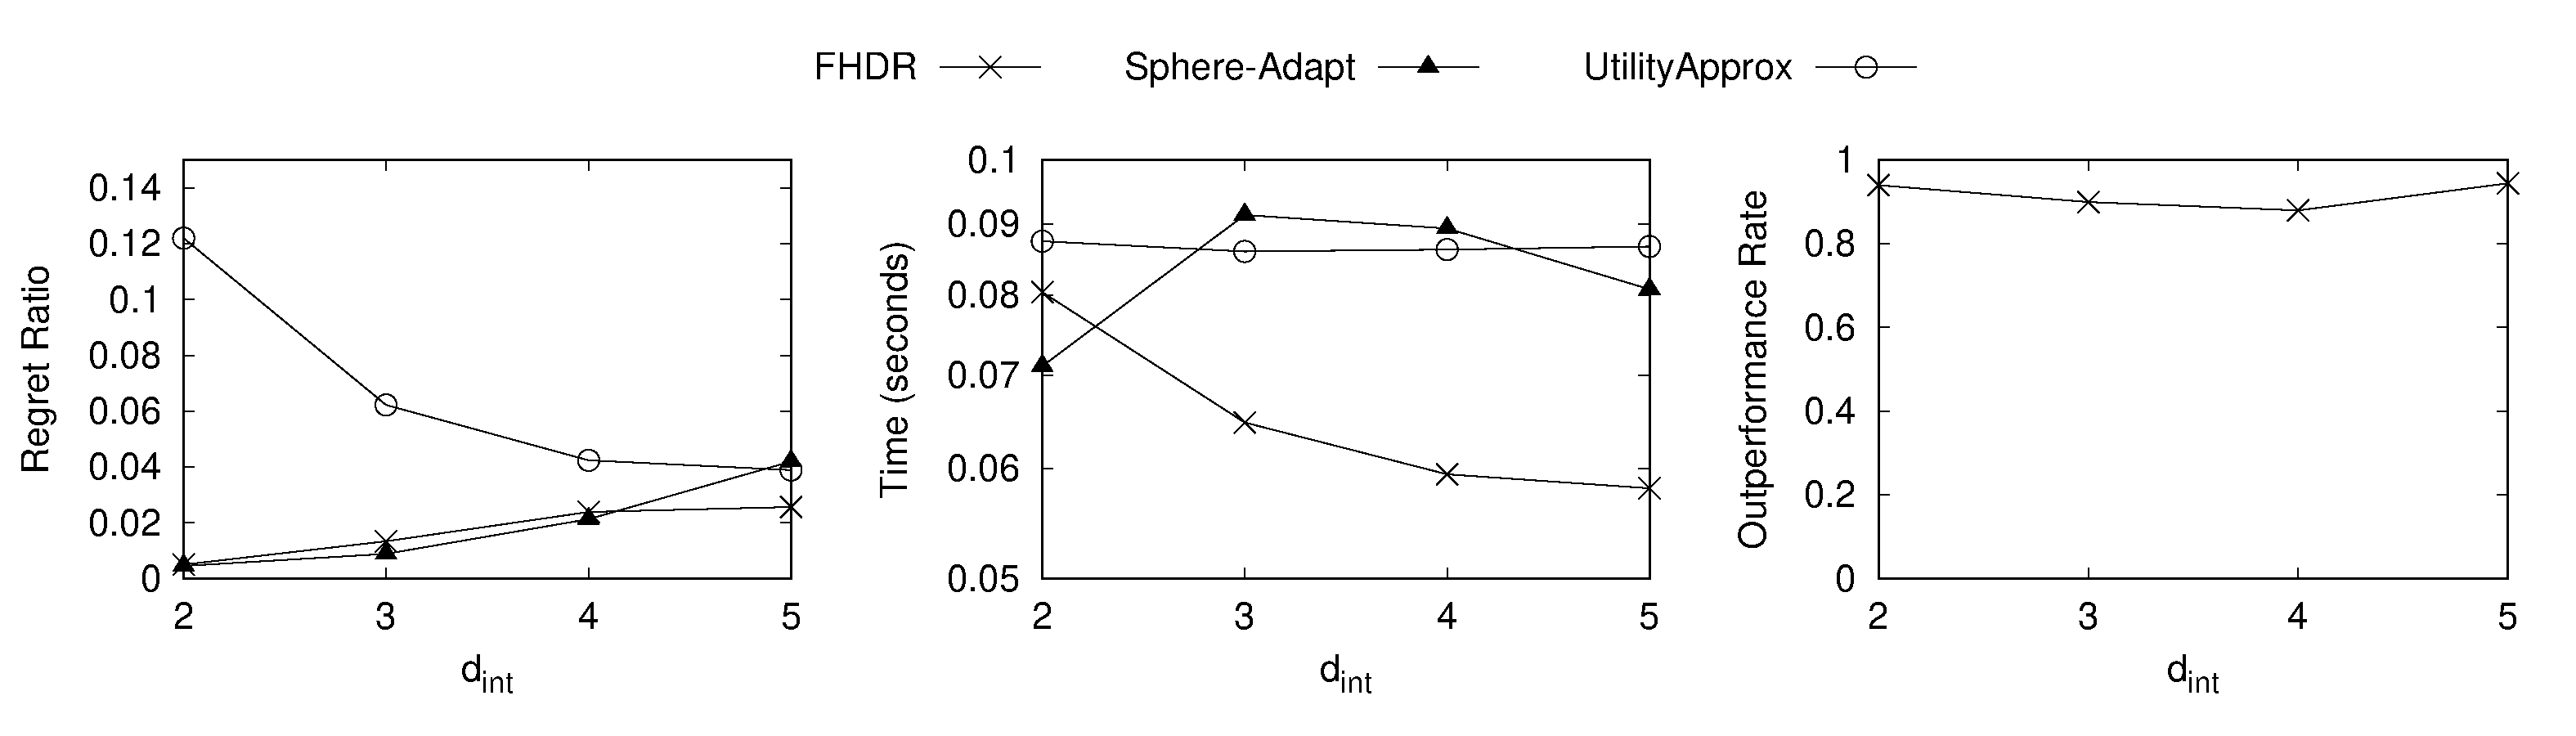
\includegraphics[width=\linewidth]{plot/real/nba/d_int_2_plots.pdf}
        \vspace{-1.5em}
        \caption{P2: Vary $d_{\text{int}}$}
        \label{fig:nba_b}
      \end{subfigure}
    
    \begin{subfigure}{\linewidth}
        \centering
        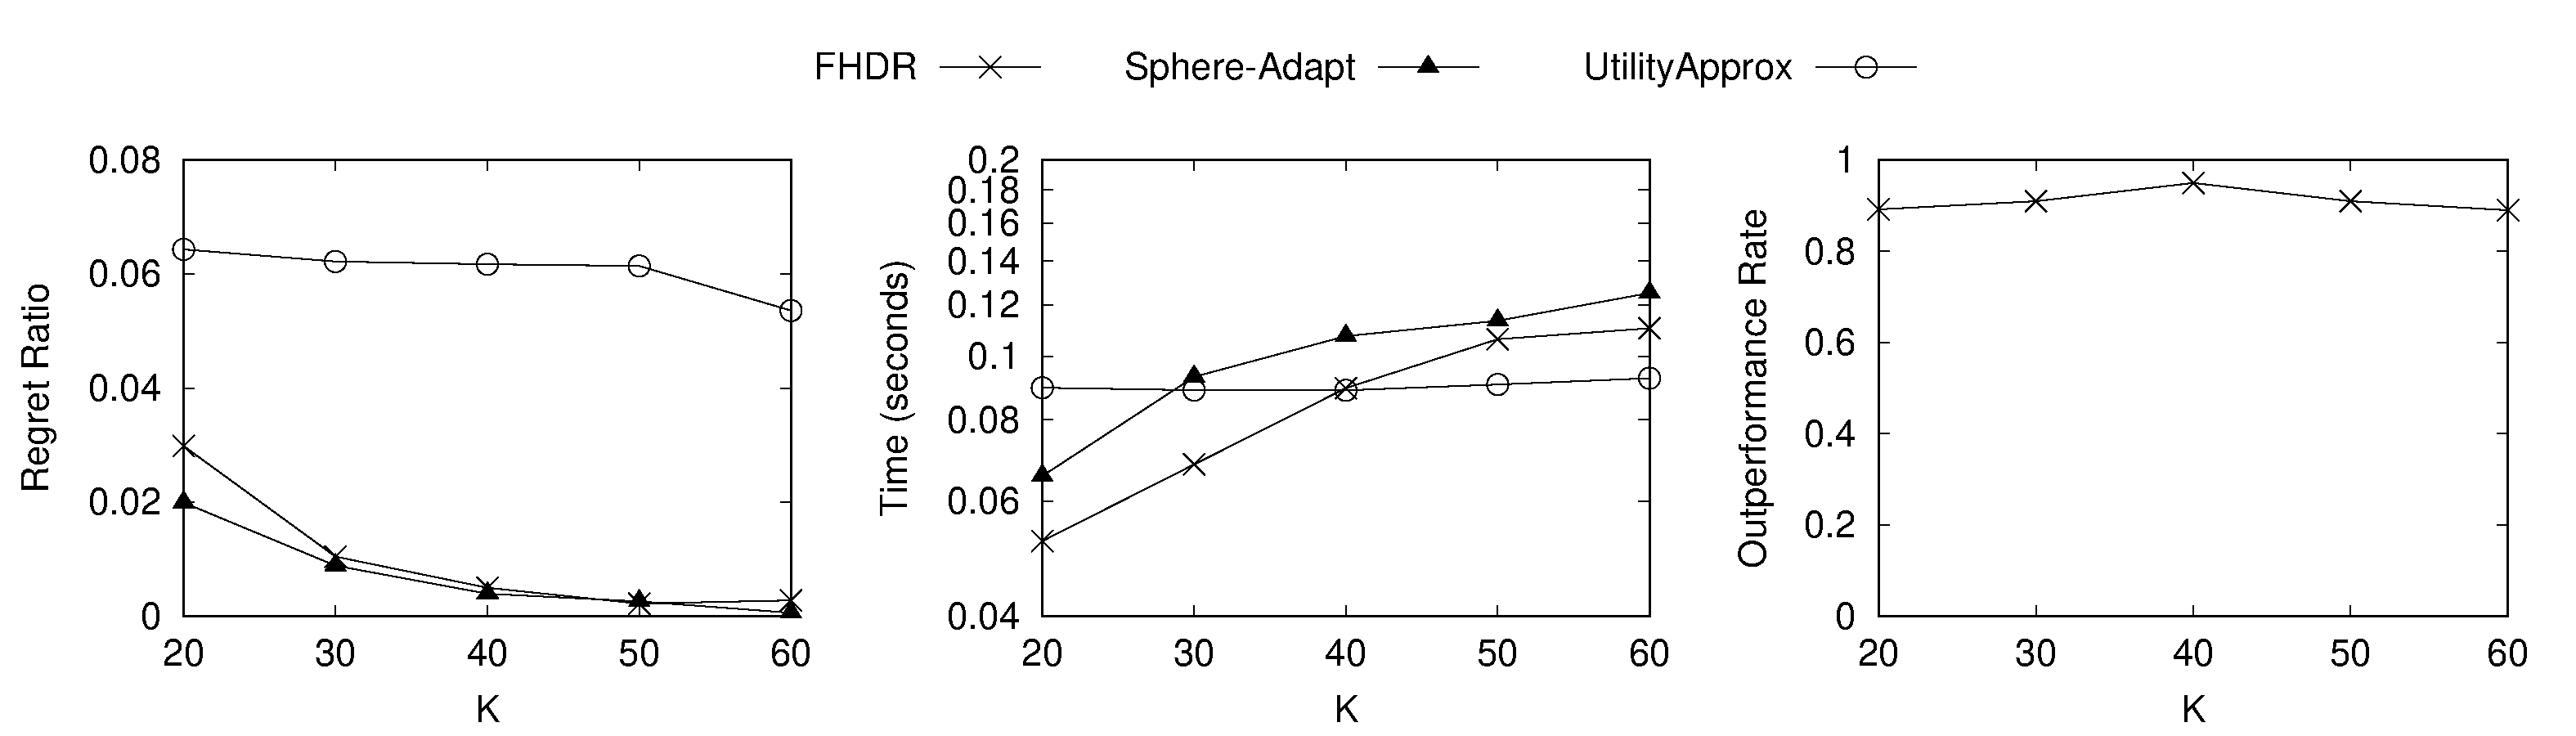
\includegraphics[width=\linewidth]{plot/real/nba/K_plots.pdf}
        \vspace{-1.5em}
        \caption{P2: Vary $K$}
        \label{fig:nba_c}
      \end{subfigure}

    \begin{subfigure}{\linewidth}
        \centering
        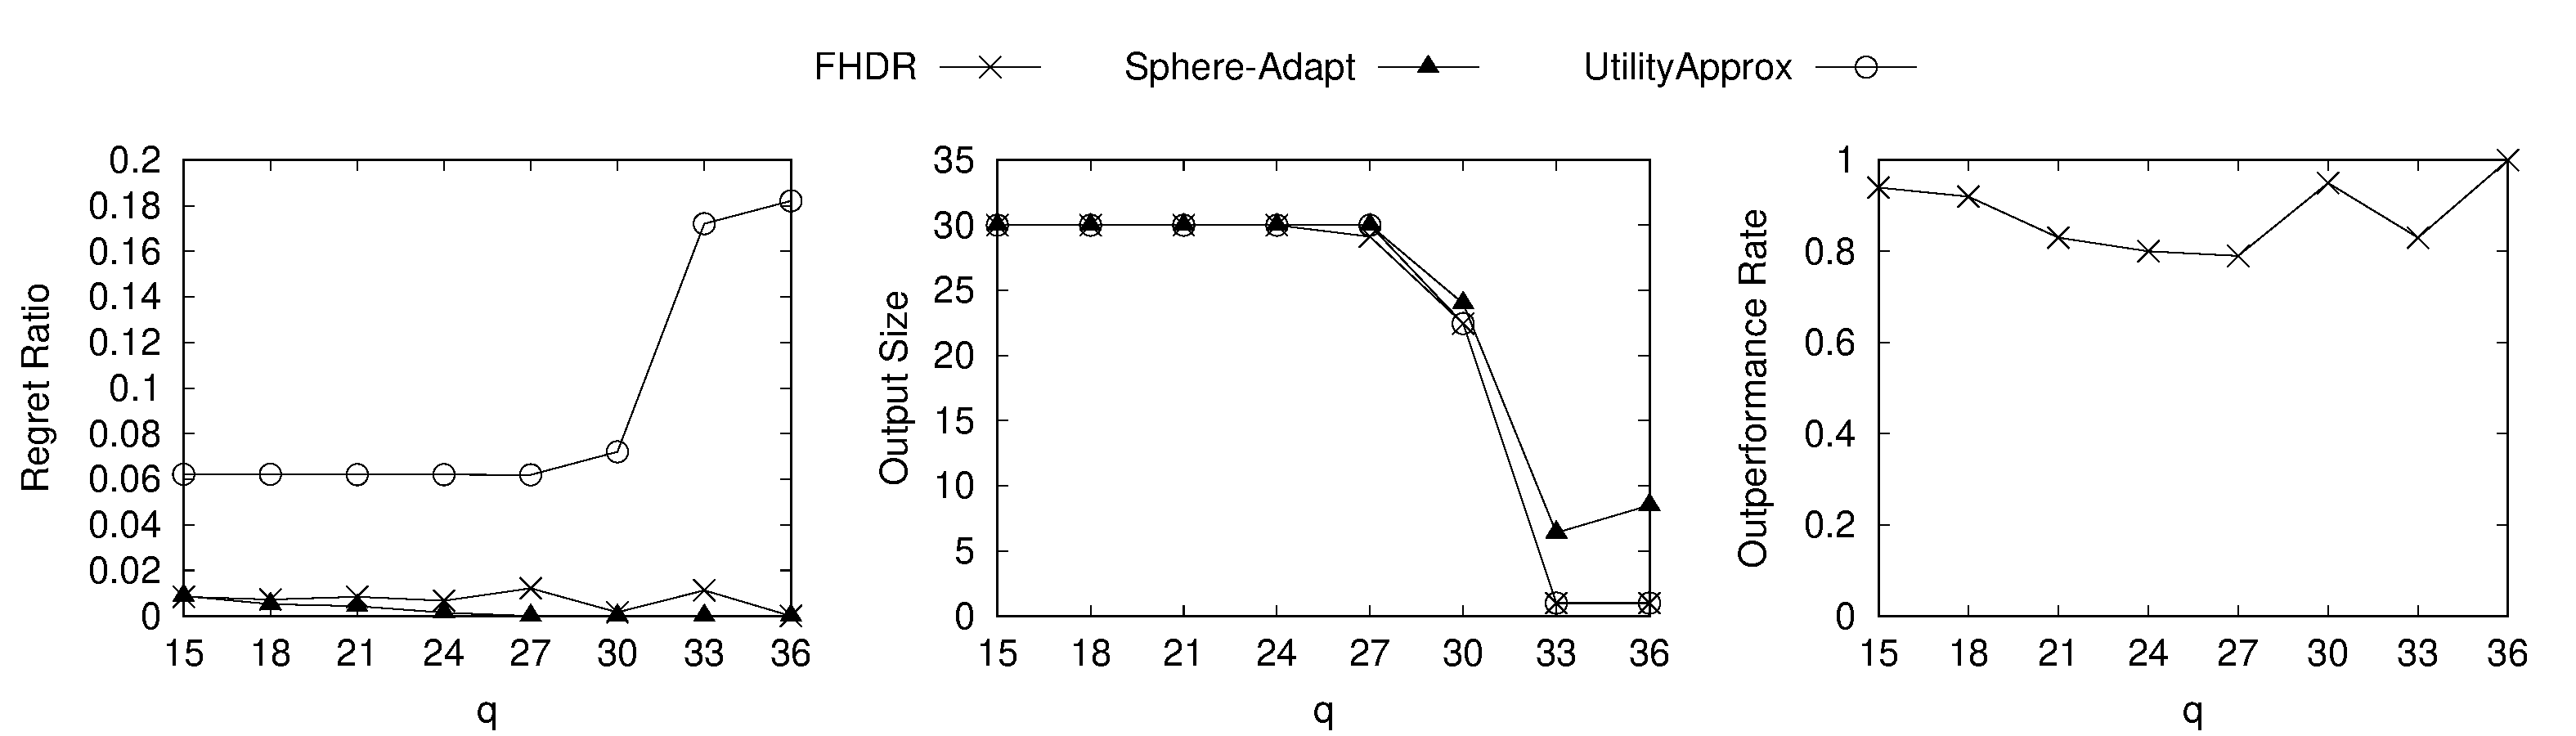
\includegraphics[width=\linewidth]{plot/real/nba/q_plots.pdf}
        \vspace{-1.5em}
        \caption{P2: Vary $q$}
        \label{fig:nba_d}
      \end{subfigure}
    
    \begin{subfigure}{\linewidth}
        \centering
        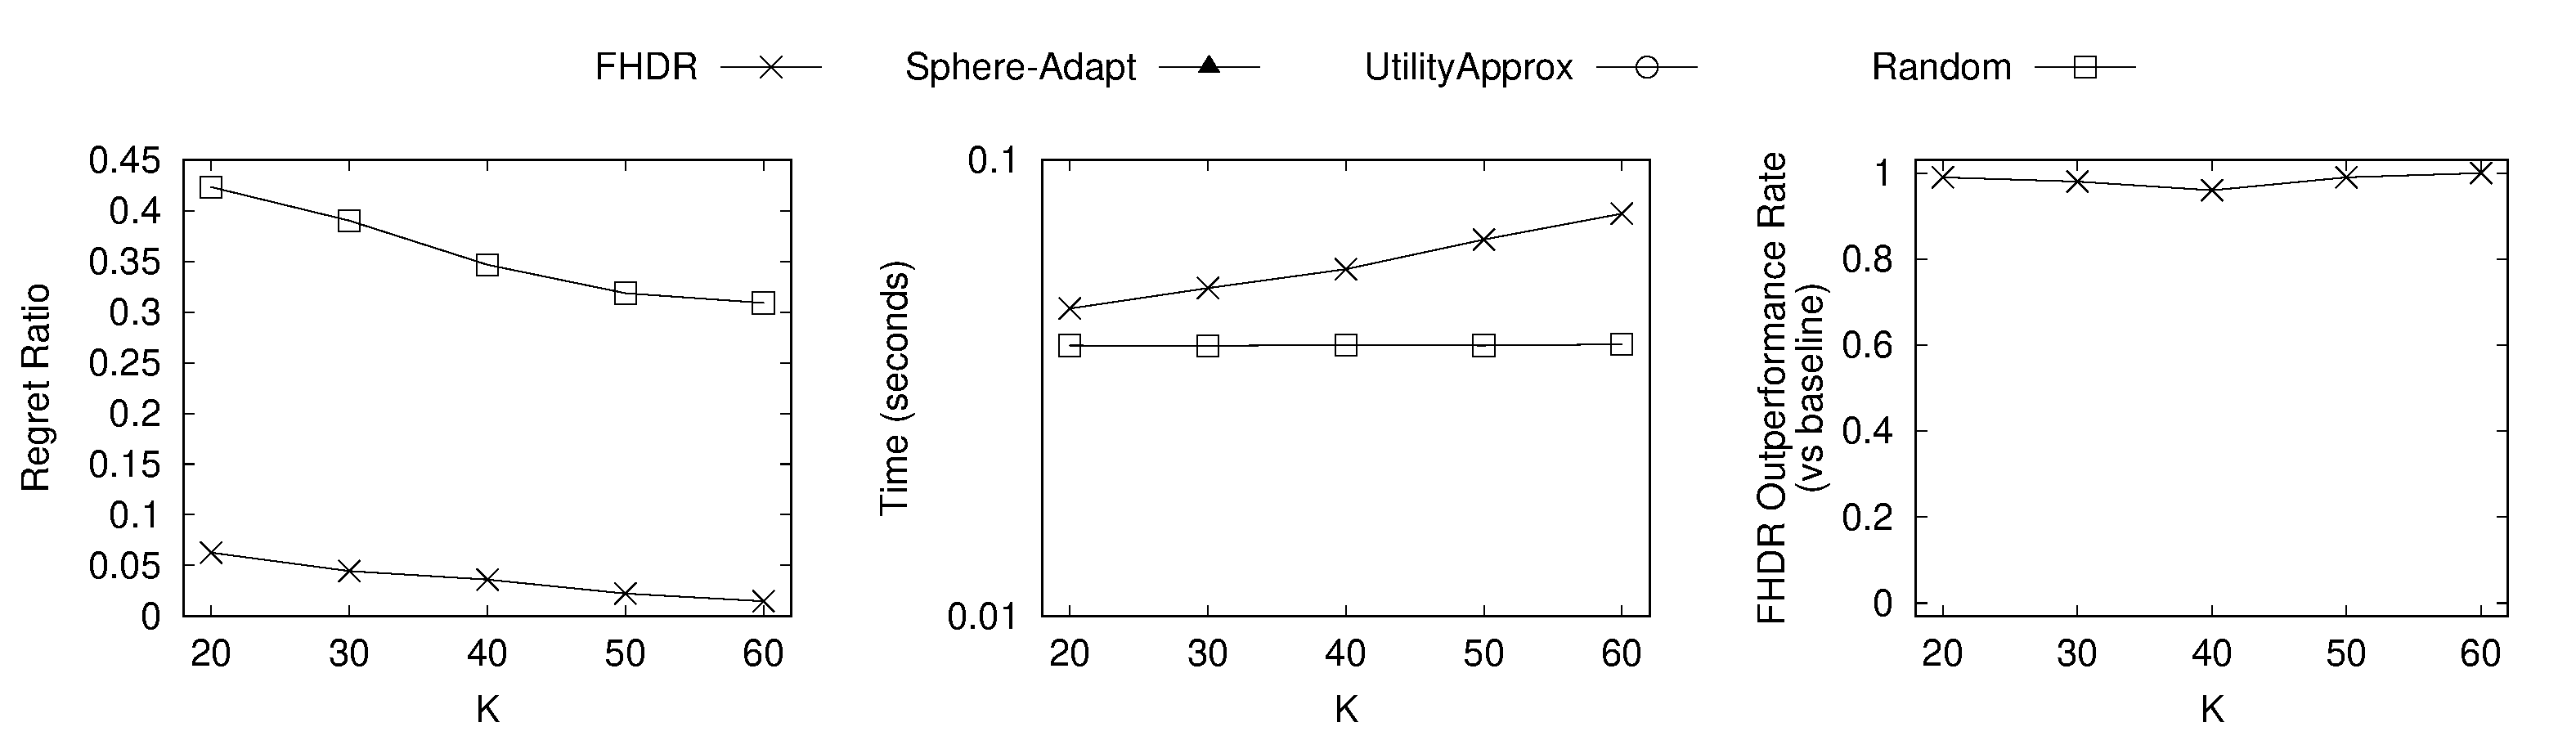
\includegraphics[width=\linewidth]{plot/p2_star/nba_K_plots.pdf}
        \vspace{-1.5em}
        \caption{$P2^{*}$: Vary $K$}
        \label{fig:p2star_nba}
    \end{subfigure}

    \caption{Results on \textit{NBA} dataset}
    \label{fig:nba}
\end{figure}

\subsection{User Study}
\label{sec:user_study}

\begin{figure}[ht]
  \centering
  \captionsetup[subfigure]{font=scriptsize,justification=centering}

  \begin{subfigure}[t]{0.48\columnwidth}
    \centering
    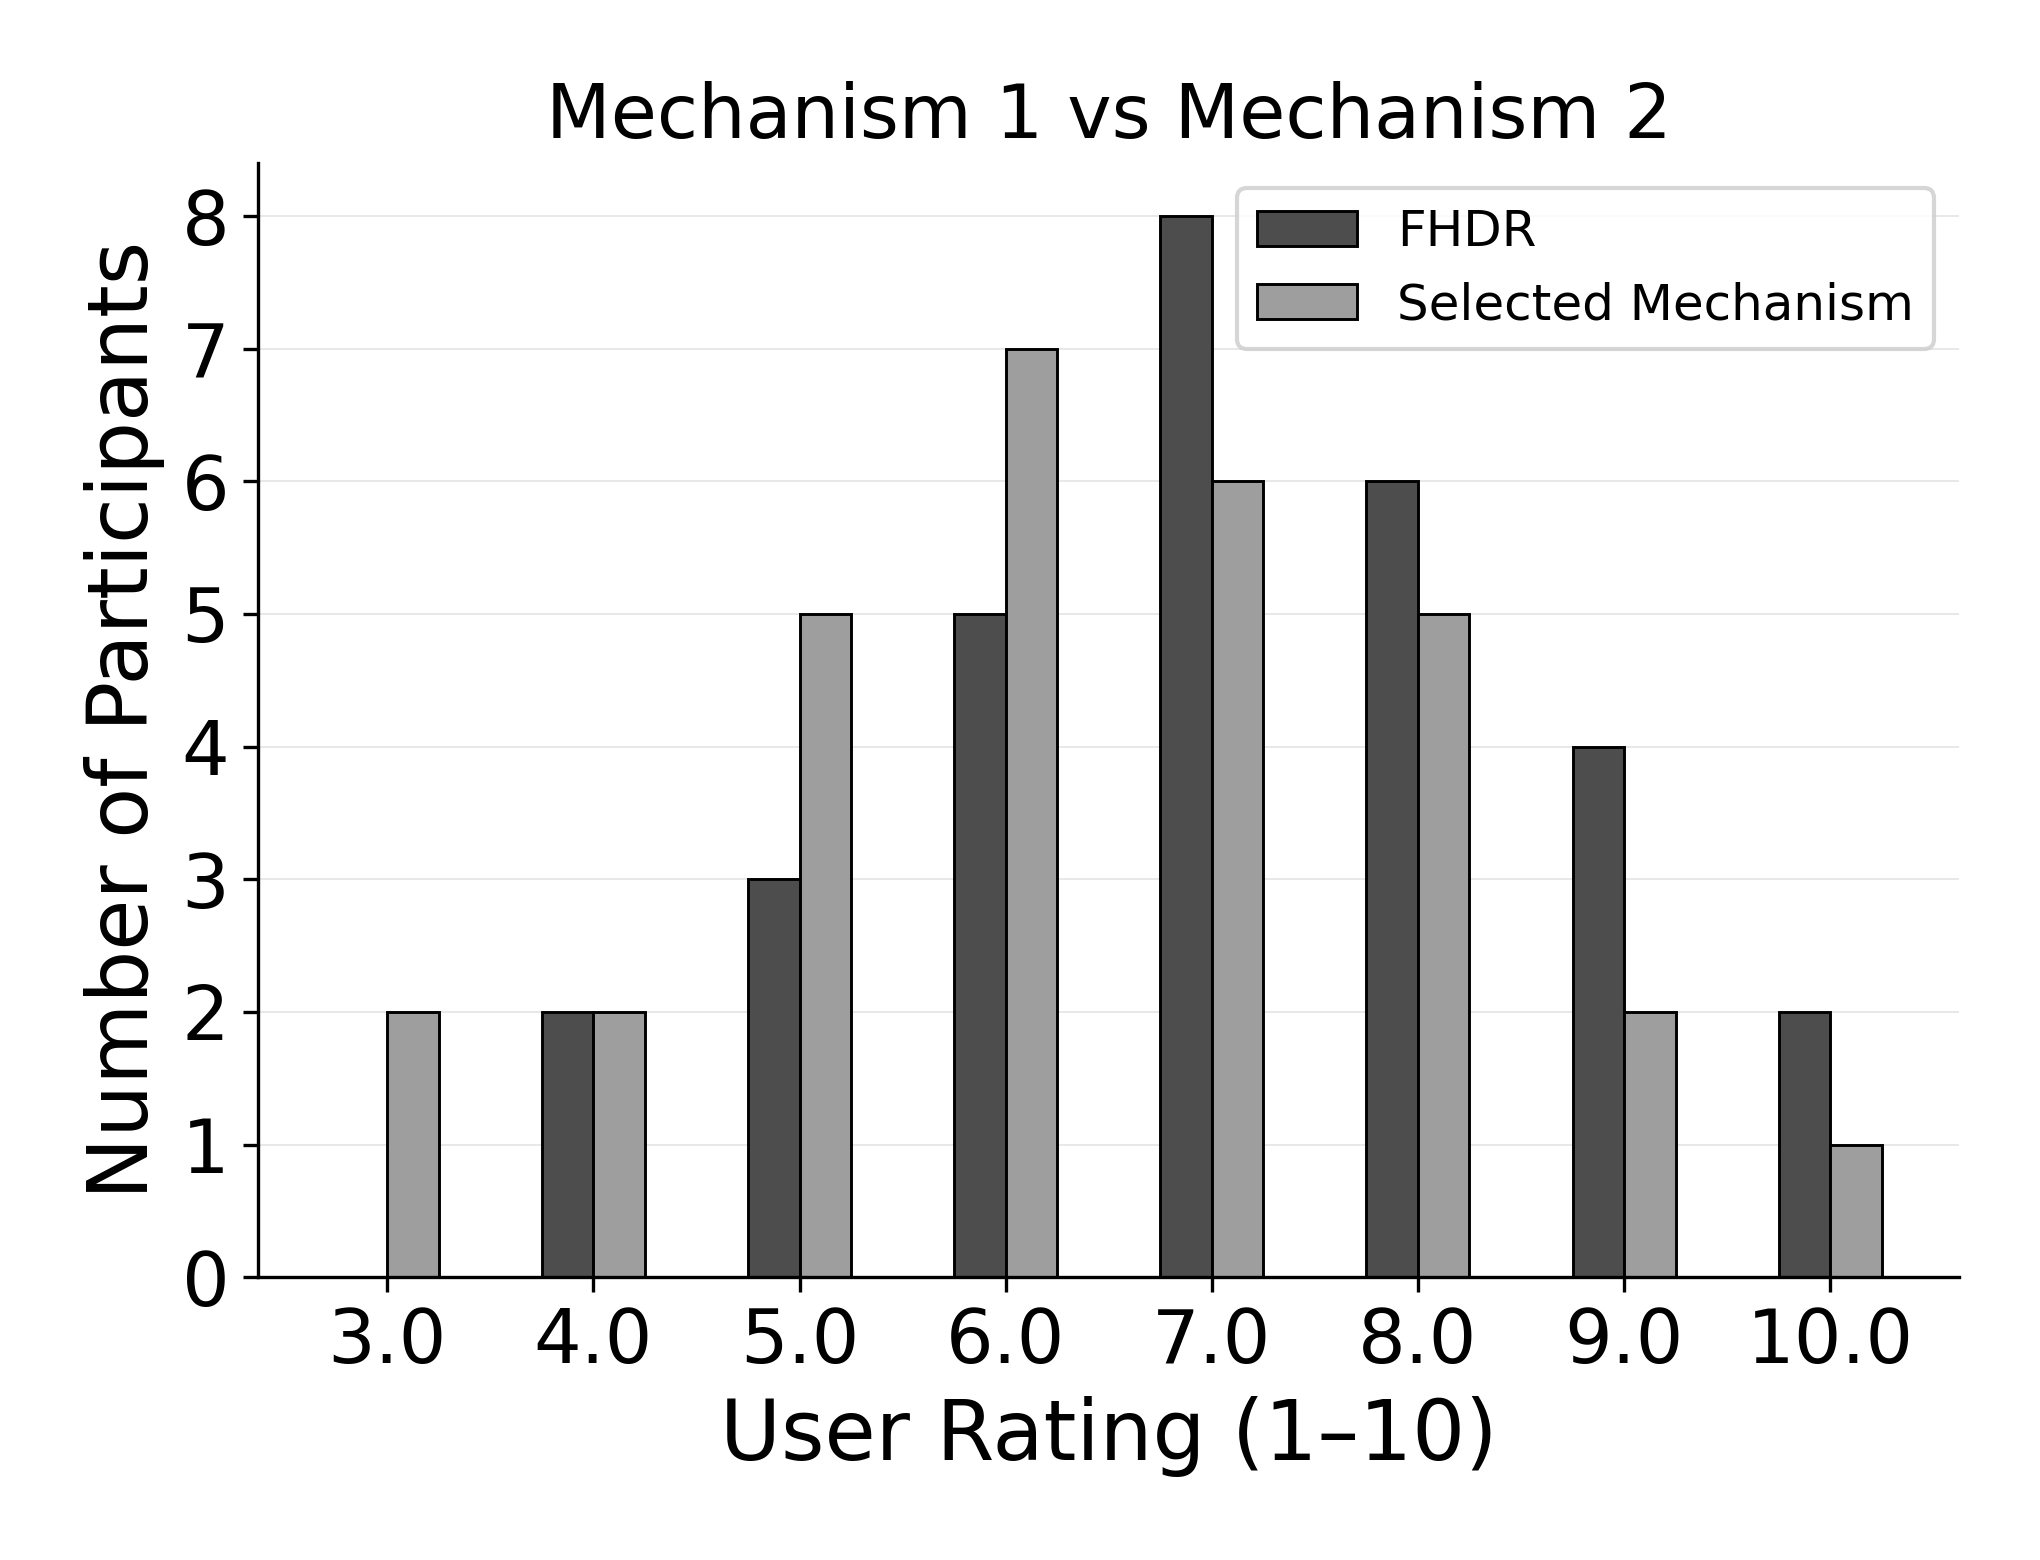
\includegraphics[width=\linewidth]{plot/user_study_2.png}
    \caption{Mechanism 1 vs.~2}
    \label{fig:userstudy_2}
  \end{subfigure}
  \hfill
  \begin{subfigure}[t]{0.48\columnwidth}
    \centering
    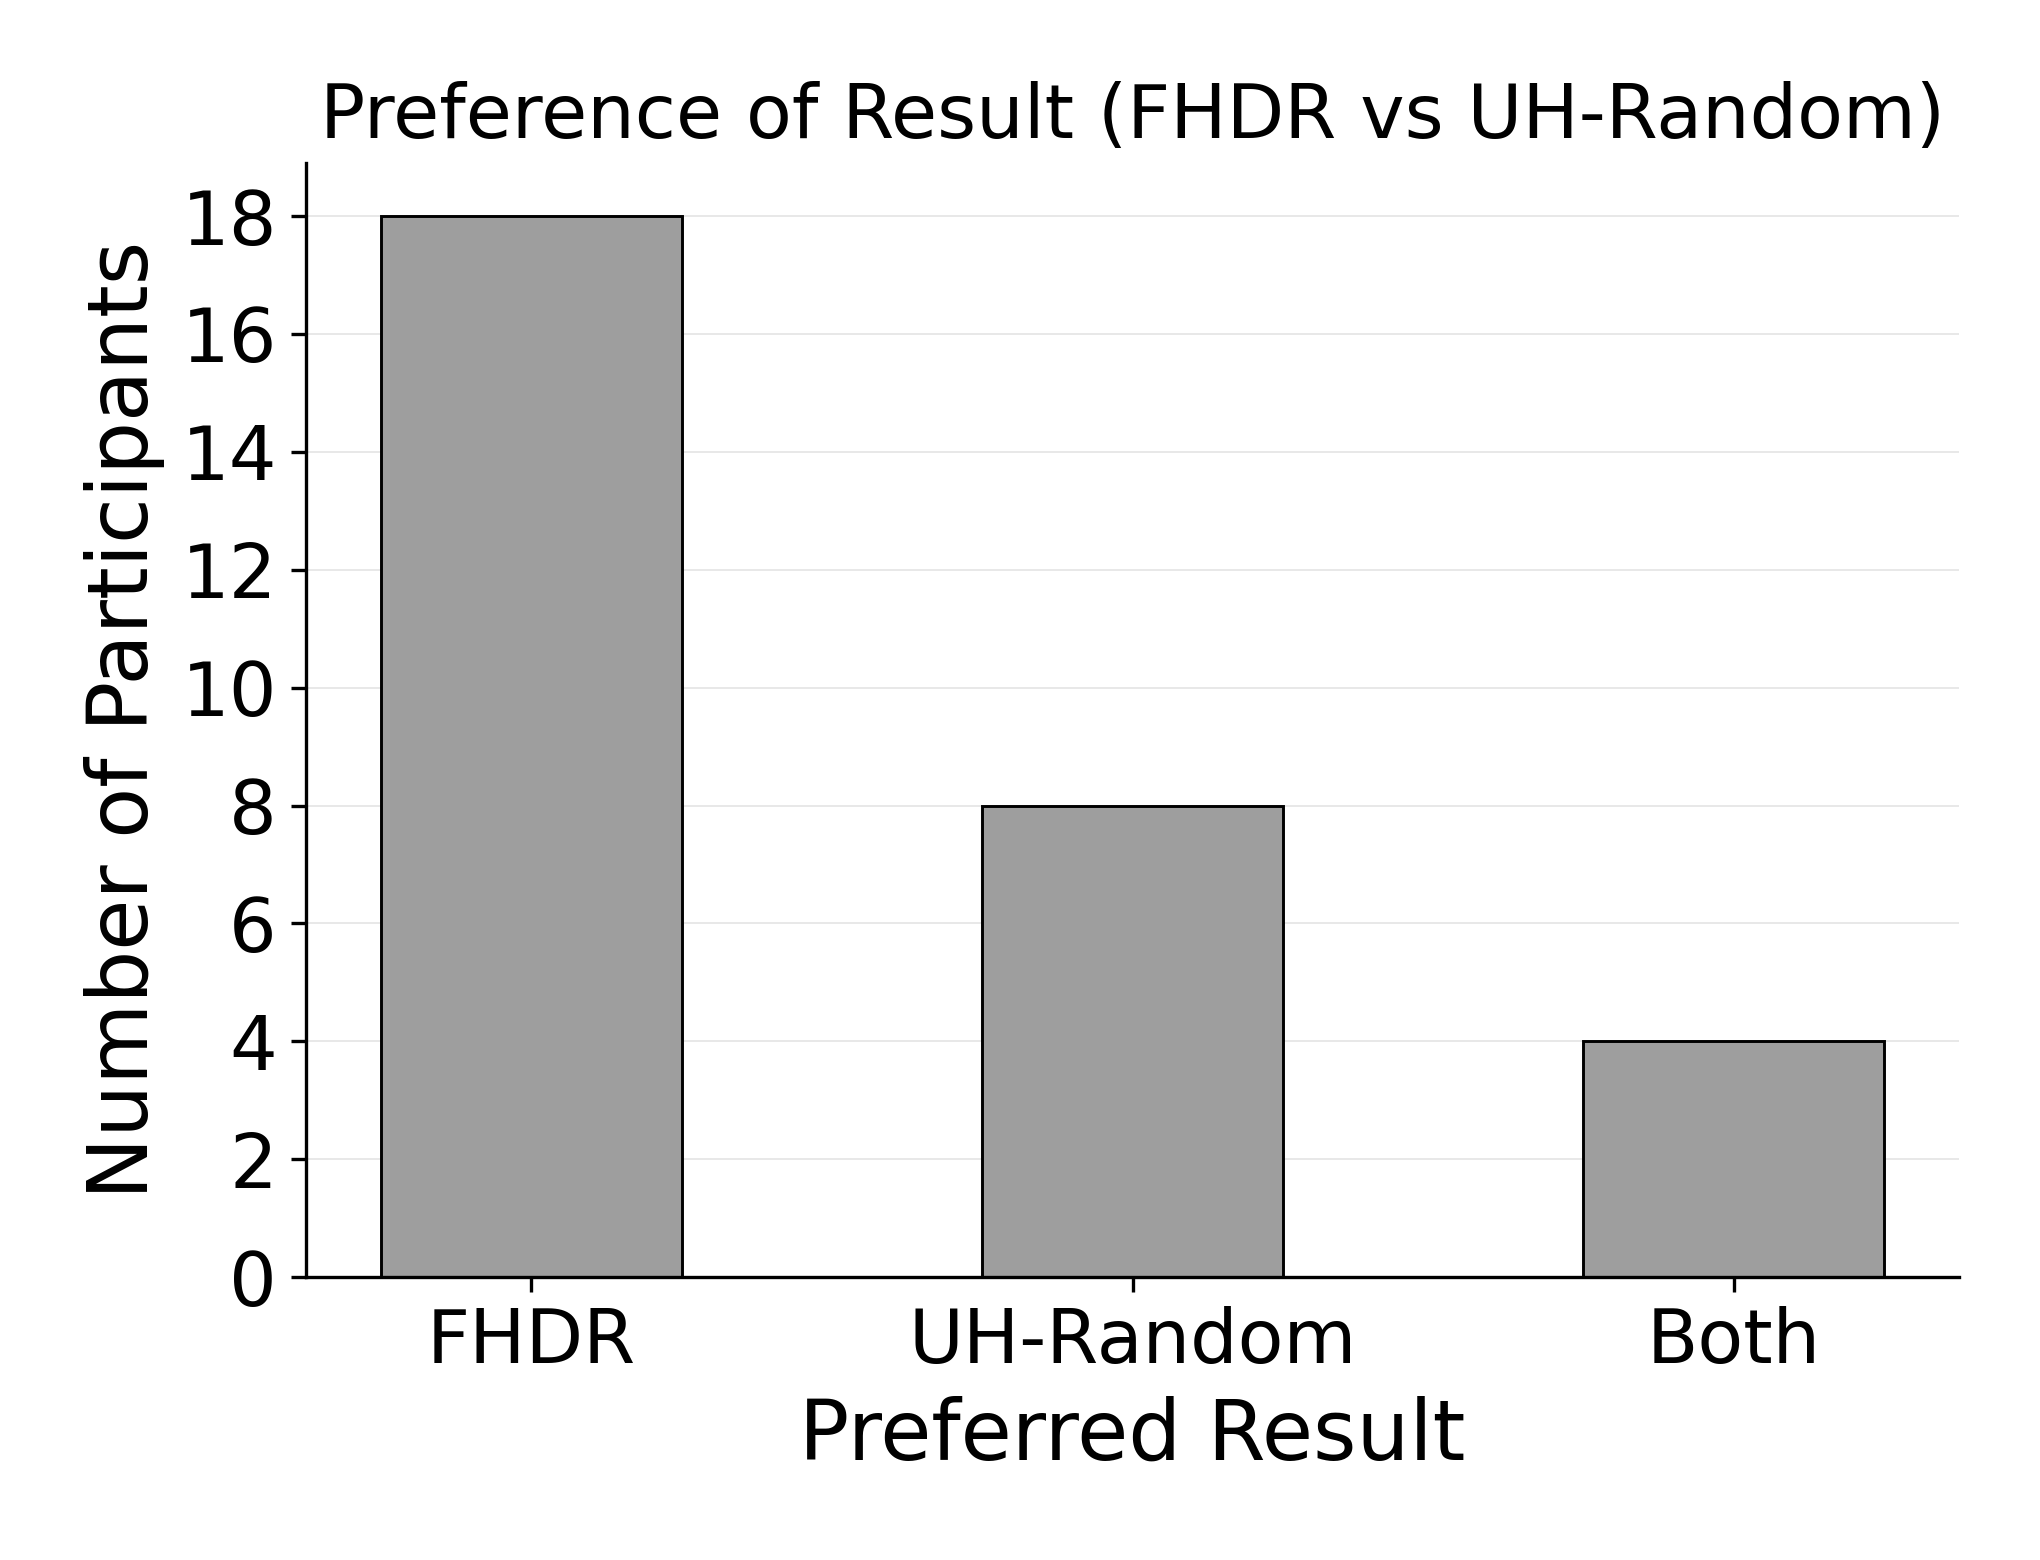
\includegraphics[width=\linewidth]{plot/user_study_3.png}
    \caption{Result preference}
    \label{fig:userstudy_3}
  \end{subfigure}

  \caption{User study results}
  \label{fig:userstudy}
  \vspace{-0.8em}
\end{figure}

We conducted a user study\footnote{Study interface: \url{https://highdim-rm-demo-production.up.railway.app/}.} on the Car dataset to evaluate the practical usability of \textsc{FHDR}, because vehicle selection is intuitive and the dataset's $57$ attributes provide a representative high-dimensional setting. The study involved the same $30$ participants as the attribute-selection survey, and the results were averaged across participants.

We compare \textsc{FHDR} with \textsc{UH-Random}, evaluating their interaction mechanisms and returned recommendations. \textsc{UtilityApprox} is excluded because it requires over $1{,}000$ questions, making a direct user-study comparison impractical. Single-round methods such as \textsc{Sphere} are excluded from this interaction-experience comparison. To reduce bias, the interface does not reveal which method is ours.

Participants interact with both methods. During each tuple comparison, the interface displays only the attributes used in that question and their values. Participants are explicitly instructed to treat omitted attributes as identical, following the interaction model in Section~\ref{sec:def}. For \textsc{UH-Random}, they select between $2$ and $7$ relevant attributes and interact with the method on the projected dataset. They then compare the recommendations and interaction mechanisms. Mechanism~1, used by \textsc{FHDR}, relies on pairwise comparisons over a small number of displayed attributes. Mechanism~2, used by \textsc{UH-Random}, requires upfront attribute selection but generally fewer subsequent questions.

Figure~\ref{fig:userstudy} summarizes the results, with detailed statistics in \iftoggle{TechnicalReport}{Section~\ref{appen:user_study} of the \technicalreport}{Appendix~\ref{appen:user_study}}. Figure~\ref{fig:userstudy_2} shows that Mechanism~1 received a higher average rating than Mechanism~2, with scores of $7.10$ and $6.37$, respectively, while Mechanism~2 exhibited greater variation. These results support the usability advantage of avoiding upfront attribute selection. In Figure~\ref{fig:userstudy_3}, $18$ participants preferred FHDR’s output, $8$ preferred UH-Random’s, and $4$ rated them as comparable.

